% Options for packages loaded elsewhere
\PassOptionsToPackage{unicode}{hyperref}
\PassOptionsToPackage{hyphens}{url}
\PassOptionsToPackage{dvipsnames,svgnames,x11names}{xcolor}
%
\documentclass[
  letterpaper,
  DIV=11,
  numbers=noendperiod]{scrreprt}

\usepackage{amsmath,amssymb}
\usepackage{lmodern}
\usepackage{iftex}
\ifPDFTeX
  \usepackage[T1]{fontenc}
  \usepackage[utf8]{inputenc}
  \usepackage{textcomp} % provide euro and other symbols
\else % if luatex or xetex
  \usepackage{unicode-math}
  \defaultfontfeatures{Scale=MatchLowercase}
  \defaultfontfeatures[\rmfamily]{Ligatures=TeX,Scale=1}
\fi
% Use upquote if available, for straight quotes in verbatim environments
\IfFileExists{upquote.sty}{\usepackage{upquote}}{}
\IfFileExists{microtype.sty}{% use microtype if available
  \usepackage[]{microtype}
  \UseMicrotypeSet[protrusion]{basicmath} % disable protrusion for tt fonts
}{}
\makeatletter
\@ifundefined{KOMAClassName}{% if non-KOMA class
  \IfFileExists{parskip.sty}{%
    \usepackage{parskip}
  }{% else
    \setlength{\parindent}{0pt}
    \setlength{\parskip}{6pt plus 2pt minus 1pt}}
}{% if KOMA class
  \KOMAoptions{parskip=half}}
\makeatother
\usepackage{xcolor}
\setlength{\emergencystretch}{3em} % prevent overfull lines
\setcounter{secnumdepth}{5}
% Make \paragraph and \subparagraph free-standing
\ifx\paragraph\undefined\else
  \let\oldparagraph\paragraph
  \renewcommand{\paragraph}[1]{\oldparagraph{#1}\mbox{}}
\fi
\ifx\subparagraph\undefined\else
  \let\oldsubparagraph\subparagraph
  \renewcommand{\subparagraph}[1]{\oldsubparagraph{#1}\mbox{}}
\fi

\usepackage{color}
\usepackage{fancyvrb}
\newcommand{\VerbBar}{|}
\newcommand{\VERB}{\Verb[commandchars=\\\{\}]}
\DefineVerbatimEnvironment{Highlighting}{Verbatim}{commandchars=\\\{\}}
% Add ',fontsize=\small' for more characters per line
\usepackage{framed}
\definecolor{shadecolor}{RGB}{241,243,245}
\newenvironment{Shaded}{\begin{snugshade}}{\end{snugshade}}
\newcommand{\AlertTok}[1]{\textcolor[rgb]{0.68,0.00,0.00}{#1}}
\newcommand{\AnnotationTok}[1]{\textcolor[rgb]{0.37,0.37,0.37}{#1}}
\newcommand{\AttributeTok}[1]{\textcolor[rgb]{0.40,0.45,0.13}{#1}}
\newcommand{\BaseNTok}[1]{\textcolor[rgb]{0.68,0.00,0.00}{#1}}
\newcommand{\BuiltInTok}[1]{\textcolor[rgb]{0.00,0.23,0.31}{#1}}
\newcommand{\CharTok}[1]{\textcolor[rgb]{0.13,0.47,0.30}{#1}}
\newcommand{\CommentTok}[1]{\textcolor[rgb]{0.37,0.37,0.37}{#1}}
\newcommand{\CommentVarTok}[1]{\textcolor[rgb]{0.37,0.37,0.37}{\textit{#1}}}
\newcommand{\ConstantTok}[1]{\textcolor[rgb]{0.56,0.35,0.01}{#1}}
\newcommand{\ControlFlowTok}[1]{\textcolor[rgb]{0.00,0.23,0.31}{#1}}
\newcommand{\DataTypeTok}[1]{\textcolor[rgb]{0.68,0.00,0.00}{#1}}
\newcommand{\DecValTok}[1]{\textcolor[rgb]{0.68,0.00,0.00}{#1}}
\newcommand{\DocumentationTok}[1]{\textcolor[rgb]{0.37,0.37,0.37}{\textit{#1}}}
\newcommand{\ErrorTok}[1]{\textcolor[rgb]{0.68,0.00,0.00}{#1}}
\newcommand{\ExtensionTok}[1]{\textcolor[rgb]{0.00,0.23,0.31}{#1}}
\newcommand{\FloatTok}[1]{\textcolor[rgb]{0.68,0.00,0.00}{#1}}
\newcommand{\FunctionTok}[1]{\textcolor[rgb]{0.28,0.35,0.67}{#1}}
\newcommand{\ImportTok}[1]{\textcolor[rgb]{0.00,0.46,0.62}{#1}}
\newcommand{\InformationTok}[1]{\textcolor[rgb]{0.37,0.37,0.37}{#1}}
\newcommand{\KeywordTok}[1]{\textcolor[rgb]{0.00,0.23,0.31}{#1}}
\newcommand{\NormalTok}[1]{\textcolor[rgb]{0.00,0.23,0.31}{#1}}
\newcommand{\OperatorTok}[1]{\textcolor[rgb]{0.37,0.37,0.37}{#1}}
\newcommand{\OtherTok}[1]{\textcolor[rgb]{0.00,0.23,0.31}{#1}}
\newcommand{\PreprocessorTok}[1]{\textcolor[rgb]{0.68,0.00,0.00}{#1}}
\newcommand{\RegionMarkerTok}[1]{\textcolor[rgb]{0.00,0.23,0.31}{#1}}
\newcommand{\SpecialCharTok}[1]{\textcolor[rgb]{0.37,0.37,0.37}{#1}}
\newcommand{\SpecialStringTok}[1]{\textcolor[rgb]{0.13,0.47,0.30}{#1}}
\newcommand{\StringTok}[1]{\textcolor[rgb]{0.13,0.47,0.30}{#1}}
\newcommand{\VariableTok}[1]{\textcolor[rgb]{0.07,0.07,0.07}{#1}}
\newcommand{\VerbatimStringTok}[1]{\textcolor[rgb]{0.13,0.47,0.30}{#1}}
\newcommand{\WarningTok}[1]{\textcolor[rgb]{0.37,0.37,0.37}{\textit{#1}}}

\providecommand{\tightlist}{%
  \setlength{\itemsep}{0pt}\setlength{\parskip}{0pt}}\usepackage{longtable,booktabs,array}
\usepackage{calc} % for calculating minipage widths
% Correct order of tables after \paragraph or \subparagraph
\usepackage{etoolbox}
\makeatletter
\patchcmd\longtable{\par}{\if@noskipsec\mbox{}\fi\par}{}{}
\makeatother
% Allow footnotes in longtable head/foot
\IfFileExists{footnotehyper.sty}{\usepackage{footnotehyper}}{\usepackage{footnote}}
\makesavenoteenv{longtable}
\usepackage{graphicx}
\makeatletter
\def\maxwidth{\ifdim\Gin@nat@width>\linewidth\linewidth\else\Gin@nat@width\fi}
\def\maxheight{\ifdim\Gin@nat@height>\textheight\textheight\else\Gin@nat@height\fi}
\makeatother
% Scale images if necessary, so that they will not overflow the page
% margins by default, and it is still possible to overwrite the defaults
% using explicit options in \includegraphics[width, height, ...]{}
\setkeys{Gin}{width=\maxwidth,height=\maxheight,keepaspectratio}
% Set default figure placement to htbp
\makeatletter
\def\fps@figure{htbp}
\makeatother
\newlength{\cslhangindent}
\setlength{\cslhangindent}{1.5em}
\newlength{\csllabelwidth}
\setlength{\csllabelwidth}{3em}
\newlength{\cslentryspacingunit} % times entry-spacing
\setlength{\cslentryspacingunit}{\parskip}
\newenvironment{CSLReferences}[2] % #1 hanging-ident, #2 entry spacing
 {% don't indent paragraphs
  \setlength{\parindent}{0pt}
  % turn on hanging indent if param 1 is 1
  \ifodd #1
  \let\oldpar\par
  \def\par{\hangindent=\cslhangindent\oldpar}
  \fi
  % set entry spacing
  \setlength{\parskip}{#2\cslentryspacingunit}
 }%
 {}
\usepackage{calc}
\newcommand{\CSLBlock}[1]{#1\hfill\break}
\newcommand{\CSLLeftMargin}[1]{\parbox[t]{\csllabelwidth}{#1}}
\newcommand{\CSLRightInline}[1]{\parbox[t]{\linewidth - \csllabelwidth}{#1}\break}
\newcommand{\CSLIndent}[1]{\hspace{\cslhangindent}#1}

\KOMAoption{captions}{tableheading}
\makeatletter
\makeatother
\makeatletter
\@ifpackageloaded{bookmark}{}{\usepackage{bookmark}}
\makeatother
\makeatletter
\@ifpackageloaded{caption}{}{\usepackage{caption}}
\AtBeginDocument{%
\ifdefined\contentsname
  \renewcommand*\contentsname{Table of contents}
\else
  \newcommand\contentsname{Table of contents}
\fi
\ifdefined\listfigurename
  \renewcommand*\listfigurename{List of Figures}
\else
  \newcommand\listfigurename{List of Figures}
\fi
\ifdefined\listtablename
  \renewcommand*\listtablename{List of Tables}
\else
  \newcommand\listtablename{List of Tables}
\fi
\ifdefined\figurename
  \renewcommand*\figurename{Figure}
\else
  \newcommand\figurename{Figure}
\fi
\ifdefined\tablename
  \renewcommand*\tablename{Table}
\else
  \newcommand\tablename{Table}
\fi
}
\@ifpackageloaded{float}{}{\usepackage{float}}
\floatstyle{ruled}
\@ifundefined{c@chapter}{\newfloat{codelisting}{h}{lop}}{\newfloat{codelisting}{h}{lop}[chapter]}
\floatname{codelisting}{Listing}
\newcommand*\listoflistings{\listof{codelisting}{List of Listings}}
\makeatother
\makeatletter
\@ifpackageloaded{caption}{}{\usepackage{caption}}
\@ifpackageloaded{subcaption}{}{\usepackage{subcaption}}
\makeatother
\makeatletter
\@ifpackageloaded{tcolorbox}{}{\usepackage[many]{tcolorbox}}
\makeatother
\makeatletter
\@ifundefined{shadecolor}{\definecolor{shadecolor}{rgb}{.97, .97, .97}}
\makeatother
\makeatletter
\makeatother
\ifLuaTeX
  \usepackage{selnolig}  % disable illegal ligatures
\fi
\IfFileExists{bookmark.sty}{\usepackage{bookmark}}{\usepackage{hyperref}}
\IfFileExists{xurl.sty}{\usepackage{xurl}}{} % add URL line breaks if available
\urlstyle{same} % disable monospaced font for URLs
\hypersetup{
  pdftitle={stats\_notes},
  pdfauthor={Jane Doe},
  colorlinks=true,
  linkcolor={blue},
  filecolor={Maroon},
  citecolor={Blue},
  urlcolor={Blue},
  pdfcreator={LaTeX via pandoc}}

\title{stats\_notes}
\author{Jane Doe}
\date{1/12/22}

\begin{document}
\maketitle
\ifdefined\Shaded\renewenvironment{Shaded}{\begin{tcolorbox}[boxrule=0pt, breakable, borderline west={3pt}{0pt}{shadecolor}, sharp corners, enhanced, frame hidden, interior hidden]}{\end{tcolorbox}}\fi

\renewcommand*\contentsname{Table of contents}
{
\hypersetup{linkcolor=}
\setcounter{tocdepth}{2}
\tableofcontents
}
\bookmarksetup{startatroot}

\hypertarget{preface}{%
\chapter*{Preface}\label{preface}}
\addcontentsline{toc}{chapter}{Preface}

\markboth{Preface}{Preface}

This is a Quarto book.

To learn more about Quarto books visit
\url{https://quarto.org/docs/books}.

\bookmarksetup{startatroot}

\hypertarget{introduction}{%
\chapter{Introduction}\label{introduction}}

This book is my personal notes for my stats course. It is very rough!

This book has been created with Quarto through VSCode. I highly
recommend it.

\bookmarksetup{startatroot}

\hypertarget{summary}{%
\chapter{Summary}\label{summary}}

In summary, this book has no content whatsoever.

\bookmarksetup{startatroot}

\hypertarget{chapter-1---intro}{%
\chapter{Chapter 1 - Intro}\label{chapter-1---intro}}

Don't forget units when reporting point or CI!

Don't report effect size if not significant!

Type 1 : False Positive, treatemnts same but report significant.
\(\alpha\) is probability of FP.

Type 2 : False Negative, treatemnts different but missed, \(\beta\) is
probability of FN.

Confidence interval of the mean

\(\bar{X} \pm t_{0.975, \nu} \frac{\sigma}{\sqrt{N}}\)

A clinical trial:

\begin{itemize}
\tightlist
\item
  Planned, not observed
\item
  On patients, not healthy people
\item
  Use inferential procedures, stats to generalise
\end{itemize}

Phases are :

\begin{itemize}
\tightlist
\item
  Phase I - Drug safety, on volunteers
\item
  Phase II - Initial Clinical, dose finding and patient safety
\item
  Phase III - Evaluation, drug vs placebo (this course)
\item
  Phase IV - Post marketing surveillance. Checking for long term side
  effects.
\end{itemize}

Placebos counter the physcological effect of having a drug/medical
attention

Blindness:

\begin{itemize}
\tightlist
\item
  Single : Patient or practioner is unaware of which treatment
\item
  Double : Both unaware
\end{itemize}

\hypertarget{bradford-hill}{%
\section{Bradford-Hill}\label{bradford-hill}}

If all met does not mean causality, just sensible tests.

\begin{itemize}
\tightlist
\item
  Temporality - Effect follows cause
\item
  Consistency - Does it happen in multiple groups (gender, countries,
  etc)
\item
  Coherence - Do controlled and observational studies agree
\item
  Strength of Association - Greater effect observed if given treatment
\item
  Biological Gradient - More agent, more effect
\item
  Specificity - does agent specifically affect what it is applied to Eg.
  cream on hand, fixes hand
\item
  Plausibility - Can it be explained mechanistically
\item
  Freedom from bias/confounders
\item
  Analgous results elsewhere - similir agents have similar results
\end{itemize}

\hypertarget{ethics}{%
\section{Ethics}\label{ethics}}

\hypertarget{medical}{%
\subsection{Medical}\label{medical}}

Trial design is key

\begin{itemize}
\tightlist
\item
  Only trial if you genuinely don't know whether one is better
\item
  Poorly planned/exexuted (eg under powered) is very unethical
\item
  Patients have informed consent
\item
  Placebos are ethical. The ethics of the population vs individual
\item
  Ethics commitee buys in
\end{itemize}

\hypertarget{publication}{%
\subsection{Publication}\label{publication}}

Alot of money at stake

\begin{itemize}
\tightlist
\item
  Avoid publication bias, only publishing good results
\item
  Journal contributors must: declare full responsibilty held over trial,
  had access to data, made decision to publish.
\end{itemize}

\bookmarksetup{startatroot}

\hypertarget{chapter-2---trial-design}{%
\chapter{Chapter 2 - Trial Design}\label{chapter-2---trial-design}}

\hypertarget{parrallel}{%
\section{Parrallel}\label{parrallel}}

k treatments, split into k groups. May aim for equal sized groups,
though not mandatory.

Requires large numbers to be sure of treatemtn effects. Robust to
withdrawls

\hypertarget{in-series}{%
\section{In Series}\label{in-series}}

All patients, recieve all k treatments in same order. Allowing for in
patient comparison.

Benefits:

\begin{itemize}
\tightlist
\item
  Patient can express preferences
\item
  Possiblity for simultaneous treatment
\end{itemize}

Issues: - Patients may naturally imporve over time, making later
treatments look better. Progressive disease act oppositely. - Carry over
effects may exist, short term effects only - Withdrawls can be
problematic - Some orders are impossible

\hypertarget{cross-over}{%
\section{Cross Over}\label{cross-over}}

Improves upon in series to account for treatment, period, carryover.

All aptients get same treatements, but groups recieve in different
order.

In the event of dropouts period one could be used as a parrallel study,
though very low powered.

Washout may be placed between treatments (no treatment window) to
minimise carryover risk.

\hypertarget{factorial-design}{%
\section{Factorial Design}\label{factorial-design}}

Investigate effect of two or more treatments (factors), by giving
combinations.

Eg 2x2. Each parient takes two drugs, where each drug has a placebo
counterpart. Could take any combination of both drugs, one drug/one
placebo, all placebo.

May be more efficent design. May also be prone to interactions, though
this is of interest.

Mean response plots are useful for visualising effects:

\begin{itemize}
\tightlist
\item
  Two parrallel lines, no interaction
\item
  One gradient increases more, quantitative interaction
\item
  opposite gradianets, qualitative interation
\end{itemize}

TODO : PRACTICE No interaction, qualitative, quantitative

\hypertarget{sequential-design}{%
\section{Sequential Design}\label{sequential-design}}

Simple form, aptients enter as pairs, and randomly allocated A or B.

Assess which is better and move onto next pair. Cumulatively aggregate
the prefference.

You will either cross a diverging boundary and stop early or reach end
point and declare no difference.

It's an ethical approach, detecting large differences quickly.

However:

\begin{itemize}
\tightlist
\item
  Need quick response times (before next pair)
\item
  Dropouts cause issues
\item
  Requires constant attention
\item
  Boundary calculation is complex
\end{itemize}

\bookmarksetup{startatroot}

\hypertarget{chapter-3---protocol}{%
\chapter{Chapter 3 - Protocol}\label{chapter-3---protocol}}

Protocol contains:

\begin{itemize}
\tightlist
\item
  Why do the trial
\item
  Patient selection/exclusion
\item
  Sample size calcs
\item
  Trial design
\item
  How response evaluated
\item
  Analysis methods
\end{itemize}

Protocol deviations are to be expected, but must be recorded. There are
two responses to deviation.

\begin{itemize}
\tightlist
\item
  Per Protocol : Just exclude any partient that deviated. Problems are,
  power loss, affects randomisation, deviation may be a result of side
  effects.
\item
  Intention to Treat : Preffered, requires patients to be retained,
  though may yield curious answers. TODO - This is puzzling p21
\end{itemize}

Can always report both!

\bookmarksetup{startatroot}

\hypertarget{chapter-4---randomisation}{%
\chapter{Chapter 4 - Randomisation}\label{chapter-4---randomisation}}

\hypertarget{historic}{%
\section{Historic}\label{historic}}

TODO p24

\hypertarget{simple-randomisation}{%
\section{Simple Randomisation}\label{simple-randomisation}}

Generate or look up sequence of numbers. Bin the numbers into equally
sized groups.

If there is surplus, eg 3 groups, 10 Rand No.~Then ignore the designated
surplus number and move to next.

Eg.

0 1 6 7 3 2 6 8 9 5 3 2 2

A : 1-3 B : 4-6 C : 7-9 0 : ignore and try again

Negative :

\begin{itemize}
\tightlist
\item
  In small trial balance can be poor
\end{itemize}

Positive :

\begin{itemize}
\tightlist
\item
  Completely unpredictable
\item
  In long run will create equal groups
\end{itemize}

\hypertarget{blocking}{%
\section{Blocking}\label{blocking}}

Blocking is where we create clusters of treatment assignments, to ensure
balanced groups.

Eg. AB, BA 0-4 = AB 5-9 = BA

Just move along the random numbers in sequence, don't do every second,
etc

Block size can be increased to make it harder to crack Eg

AABB, ABBA, ABAB, BBAA, BABA, etc

Blocking may be crackable with small block sizes and thus may risk
double blindness.

Blocking can also be used for imbalance setting.

Block size should be as large as possible to minimise risk of cracking.
But not so large that the last block would be highly imbalanced if split
as it reached the end.

\hypertarget{stratified-randomisation}{%
\section{Stratified Randomisation}\label{stratified-randomisation}}

TODO : Watch the video on this and verify below notes (I'm 99\% sure
they are good)

Treatment (control included) groups should be as equal as possible in
terms of patient characterirstics (Age, gender, etc). Imblances could
confound treatments with characteristics. Solve with stratified
randomisation.

Say we have M/F, Over, under 50

\begin{longtable}[]{@{}ll@{}}
\toprule()
Cat. & Schema \\
\midrule()
\endhead
M, \textless50 & A B B A B B A A \\
F, \textless50 & B A B A B A A B \\
M, \textgreater50 & A B A B B A A B \\
F, \textgreater50 & A B A B A B B A \\
\bottomrule()
\end{longtable}

Instead of now applying patient count numbers, we move through the list
of patients (which should itself be random), sequentially crossing off
as we go.

\hypertarget{minimisationadaptive-randomisation}{%
\section{Minimisation/Adaptive
randomisation}\label{minimisationadaptive-randomisation}}

Where there are lots of factors strification can become impractical.

Minimisation is dynamic assignment of patients to different treatments
to achieve.

Steps:

\begin{enumerate}
\def\labelenumi{\arabic{enumi})}
\tightlist
\item
  Create a table where first column is characteristics, second col is
  factor, all other columns are treatment tallys for the characteristics
\item
  Sum down the columns and look for lowest score
\item
  Add the patient to that group and update the tally
\item
  Repeat
\item
  If score are equal, randomise.
\end{enumerate}

This is not truely random and could lead to a level of prediction if the
assignent history is known. To add randomisation you might add a
probability of assignment to the smaller so if it is smaller there is
some p between 0.5 and 1 whether it is assigned

\bookmarksetup{startatroot}

\hypertarget{chapter-5---hypothesis-testing}{%
\chapter{Chapter 5 - Hypothesis
Testing}\label{chapter-5---hypothesis-testing}}

``A null hypothesis which will be adopted unless there is significant
evidence from the data that the alternate hypothesis is more viable.''

The test statistic has a sampling distribution, under the assumption
\(H_0\) is true.

Calculate the proability that the test statistics is as or more extreme
than that observed. This is done with the sampling distribution.

The course has the following convention for the significance probability
(p-value)

\begin{longtable}[]{@{}ll@{}}
\toprule()
p-value & statement \\
\midrule()
\endhead
p\textgreater0.1 & No evidence against \(H_0\) \\
0.05\textless p\textless0.01 & Weak evidence against \(H_0\) \\
0.05\textless p\textless0.01 & Some evidence against \\
0.05\textless p\textless0.01 & Strong evidence against \\
p\textless0.001 & Very strong evidence against \\
\bottomrule()
\end{longtable}

In this course a conclusion should be as follows:

\begin{itemize}
\tightlist
\item
  Identify evidence strength verbally and quote p-value
\item
  State the null hypothesis you are rejecting, without using the words
  Null Hypothesis / \(H_0\). Use a description.
\item
  Do not convert \(H_0\) inadvertently to one-sided test
\item
  State the direction of change and a mean (point value)
\item
  Provide confidence intervals if significant
\end{itemize}

Care should be taken with p-value: - Even with substantial evidence,
alternative may not actually be true - An effect can be statistically
significant, but be too small to matter IRL - A large p-value does not
mean alterbative is wrong. Could have two little data, poor design or by
chance

Tests have assumptions!

\hypertarget{two-sample-t-test}{%
\section{Two-Sample T-Test}\label{two-sample-t-test}}

One sample required if:

\begin{itemize}
\tightlist
\item
  Comparing matched groups (difference from 0)
\item
  Comparing to a baseline, fixed value
\end{itemize}

\begin{enumerate}
\def\labelenumi{\arabic{enumi})}
\item
  Identify continuous
\item
  Declare independence and that population variance not known
\item
  Declare a two sample t-test
\item
  Identify subscripts with ``Let X be''
\item
  Write that \(H_0 : \mu_X = \mu_Y\) and \(H_A : \mu_X \neq \mu_Y\)
\item
  Calculate N, \(\bar{X}\) and \(S^2_X\)
\item
  Calculate \(\nu = min(N_X, N_Y)\)
\item
  Calulate test statistic
  \(T = \frac{\bar{X} - \bar{Y}}{\sqrt{\frac{S_X^2}{N_X} + \frac{S_Y^2}{N_Y}}}\)
\item
  \(T \sim t_{\nu}\)
\item
  Look up p value in tables (either neg or pos), DOUBLE IT, it's two
  sided \(P( |t_{\nu}| > T)\)
\item
  Calulate the mean delta and find 95\% (0.025-0.975) CI
\end{enumerate}

As N gets big, t tends to normal, therefore 1.96 (approx. 2) becomes CI
multiplier

Assume normally distributed and independent samples

\hypertarget{chi-square-test}{%
\section{Chi-Square Test}\label{chi-square-test}}

Uses:

\begin{itemize}
\tightlist
\item
  Comparing two dicscrete groups
\item
  Deciding whether two factors are independent
\item
  Test a theory, eg. something can be modelled as a set ratio
\end{itemize}

\begin{enumerate}
\def\labelenumi{\arabic{enumi})}
\tightlist
\item
  Identify count based and that \(\chi_2\) appropriate
\item
  Calculate all row and column totals. Calculate overall total
\item
  Calulate each
  \(e_{ij} = \frac{\text{row total}\times \text{col total}}{\text{Overall Total}}\)
\item
  Calulate \(\frac{(o_{ij}-e_{ij})^2}{e_{ij}}\)
\item
  Sum them to get the test stat \(X^2\)
\item
  State that \(X^2 \sim \chi^2_{\nu}\)
\item
  \(\nu = (\text{n row - 1})\times (\text{n col - 1})\)
\item
  This is a one sided test due to squaring!
\item
  Convert the coloumns from counts to percents of column total for
  reporting
\end{enumerate}

TODO: Not worked beyond 5.4

\hypertarget{further-notes}{%
\section{Further Notes}\label{further-notes}}

\hypertarget{multiple-testing}{%
\subsection{Multiple Testing}\label{multiple-testing}}

Just comparing two groups relies heavily on well balanced randomisation.

Using multiple regression we can include and therefore account for
covariates (prognostic factors), this is called an ANCOVA (Analysis of
Covariance)

\hypertarget{one-vs-two-sided-tests}{%
\subsection{One vs Two sided tests}\label{one-vs-two-sided-tests}}

Always, unless very strong \textbf{prior} knowledge, use a two sided
test. One sided are more powerful.

Eg. If you think something will decrease and go one sided, but it
actually increased you would miss it, potentailly missing a harmful
effect.

\hypertarget{pooled-or-seperate-variance}{%
\subsection{Pooled or seperate
variance}\label{pooled-or-seperate-variance}}

Always seperate on the course:

\begin{itemize}
\tightlist
\item
  If you use seperate and they are the same you will still get an
  unbiased estimateof common variance
\item
  This case would result in more DoF from welch approx, however this is
  slightly more conservative anyway
\item
  However using pooled when not can get you very different DoF, whether
  pessimistic/optimistic is not possible to know without calcs
\end{itemize}

We use pooled on power tests otherwise it become impractical to assess.

\hypertarget{testing-for-equality-of-variance}{%
\subsection{Testing for equality of
variance}\label{testing-for-equality-of-variance}}

Don't:

\begin{itemize}
\tightlist
\item
  Low powered tests
\item
  Non-sig does not mean equal, only weak evidence
\item
  If doing one test followed by another you are multiple testing ? TODO
  - p44 confusing answer I think hinting at multiple testing
\end{itemize}

TODO 5.6

\bookmarksetup{startatroot}

\hypertarget{chapter-6---power}{%
\chapter{Chapter 6 - Power}\label{chapter-6---power}}

Essential ethically:

\begin{itemize}
\tightlist
\item
  Too few, low power, study could be waste
\item
  Too mnay, excessive number of people exposed
\end{itemize}

Six steps:

\begin{enumerate}
\def\labelenumi{\arabic{enumi})}
\tightlist
\item
  Declare trial type (usually parralel)
\item
  Describe outcome \(\mu\) or \(\theta\) in most of what we do
\item
  Describe end test eg. two sample t-test
\item
  Declare baseline \(\mu\) or \(\theta\)
\item
  Declare CRD (Clinical Relevant Difference) Eg. \(\mu_X - \mu_Y\)
\item
  Set Power , \(1- \beta\)
\item
  Calculate n, \textbf{remember it is per group!}
\end{enumerate}

Useful notes:

\begin{itemize}
\tightlist
\item
  \(\Phi^{-1}(\beta)\) and \(\Phi^{-1}(\frac{\alpha}{2})\) will be
  negative for sensible values
\item
  In one sided testing \(\Phi^{-1}(\frac{\alpha}{2})\) becomes
  \(\Phi^{-1}(\alpha)\)
\item
  In the binomial case \((\theta_1 - \theta_2)^2\) drives the equation.
  Therefore to detect a half smaller change requires 4 times the
  population.
\end{itemize}

Some lessons from assignment:

\begin{itemize}
\tightlist
\item
  Always \(\Phi\) not \(\phi\) when doing inv norm cdf
\item
  Explain why you round up
\item
  Don't automatically account for dropouts, only if asked
\end{itemize}

\bookmarksetup{startatroot}

\hypertarget{chapter-7---multiplicity}{%
\chapter{Chapter 7 - Multiplicity}\label{chapter-7---multiplicity}}

Key takeaways:

\begin{itemize}
\item
  You can break most rules, IF, you declare in protocol -Bonferonni is
  very poor when results corrrelated.
\item
  Multiple Endpoints
\item
  Subgroup Analysis
\item
  Interim Analysis
\item
  Multiple Regression
\item
  Repeated Measures
\end{itemize}

Increases risk of false positives. Medical trials are very expensive and
ethically can only look at so many people, so tempting to fish.

In one test the p-value controls false positve risk. However in multiple
tests, the problem becomes at least one.

A 95\% chance of not making an error, then two tests not making an error
is \(0.95^2 = 0.9025\), so about 1 in 10 and so on. For 10 this becomes
40\%. The general formula is, for k tests:

\(1-(1-\alpha)^k\)

Bonferonni correction is extremely conservative correctiuon based on
rearranging it. The correction is:

\(\frac{\alpha}{k}\)

\hypertarget{multiple-end-points}{%
\subsection{Multiple End Points}\label{multiple-end-points}}

Apply a therapy and assess multiple outcomes. Eg Give new heart meds,
measure pulse, bp standing, bp sitting, etc

\begin{itemize}
\tightlist
\item
  Could apply bonferooni, but alot might be correlated. So the could get
  lots of low p-values but all rejected
\item
  In the protocal, declare very limited responses of interest and focus
  test on these. Caputure and assess others though to verify nothing
  worrying
\item
  Multivariate analysis can handle much of the issues of correlation and
  multiplicity, however very hard to use
\end{itemize}

\hypertarget{sub-group-analysis}{%
\subsection{Sub Group Analysis}\label{sub-group-analysis}}

Sub groups are patient characteristics. Eg. Age brackets, gender, etc.

Again, only acceptable to favour one if declared in the protocol.

Again, you should still study the sub-groups and may wish to use it to
inform further research.

Could use:

\begin{itemize}
\tightlist
\item
  Bonferroni adjustment, again conservative, though seperate subgroups
  tend to be less correlated than end points
\item
  Use ANOVA across groups, but this only tells you if one is different
  in the mean
\item
  If sig detected follow up with additional tests Eg. Dunnets, Tukey
  Multiple Range
\end{itemize}

As well as splitting, we must be very careful doing post hoc
combinations. PROTOCOL!

\hypertarget{interim-analysis}{%
\subsection{Interim Analysis}\label{interim-analysis}}

Analysing as data streams in from trials.

May want to do it as:

\begin{itemize}
\tightlist
\item
  Check protocol for adherence
\item
  Catch side effects early
\item
  Provide feedback, stakeholder engaement
\item
  Catch large effects early, ethical. You would want an extremely low
  p-value to justify.
\end{itemize}

When adding more data and repeating the tests we do not use bonferroni
as not independent, other more complicated methods are used.

DECLARE INTERIM CHECK IN PROTOCOL

\hypertarget{multiple-regression}{%
\subsection{Multiple Regression}\label{multiple-regression}}

In multiple regression we typically don't worry about multiplicity, we
have purposely chosen to include them.

Problematic when we either just chuck everything in to see what happens.
Especially with interactions and high order interactions, the number of
variables can balloon.

Solution:

\begin{itemize}
\tightlist
\item
  Use domain knowledge to inform model, create interactions a priori
\item
  Use bonferonni
\end{itemize}

\hypertarget{repeated-measures}{%
\subsection{Repeated Measures}\label{repeated-measures}}

Measuring an outcome, on the same person, over time. Eg blood
concentration at 1,4,8,16 hours.

You can solve using:

\begin{itemize}
\tightlist
\item
  Summary stats designed for repeat measures Eg. Area Under Curve (AUC)
\item
  Bonferroni (highly correlated though).
\item
  Multivariate analysis that models correlation
\end{itemize}

\hypertarget{chapter-8---crossover}{%
\section{Chapter 8 - Crossover}\label{chapter-8---crossover}}

NOT ON THE FORMULA SHEET!!!!!

Crossover trials offer more efficiency over parrallel due to within
patient comparisons.

Two groups recieve two treatments but at different periods.

Possible obsevred effects include:

\begin{itemize}
\tightlist
\item
  Treatment effects, what we are trying to find, a difference in
  treatments
\item
  Period effect, different responses between periods could be due to
  seasonal effects or all patients improving over time
\item
  Carryover (also know as treatement x period interaction)
\end{itemize}

TODO - 8.2

\begin{longtable}[]{@{}lll@{}}
\toprule()
Groups & Period 1 & Period 2 \\
\midrule()
\endhead
Group 1 & A , \(Y_{11k}\) & B , \(Y_{12k}\) \\
Group 2 & B , \(Y_{21k}\) & A , \(Y_{22k}\) \\
\bottomrule()
\end{longtable}

We model the following:

\begin{itemize}
\tightlist
\item
  \(\mu\) - overall mean
\item
  \(\tau_A , \tau_B\) - Treatment effects
\item
  \(\pi_1, \pi_2\) - Period effects
\item
  \(\lambda_1, \lambda_2\) - carryover effects
\item
  \(\alpha_k\) random patient effect \(\sim N(0, \phi^2)\) between
  patients
\item
  \(epsilon_{ijk}\) independent random error
\end{itemize}

\(\alpha\) and \(\epsilon\) disappear by taking expectations

From this we can conclude that:

\begin{longtable}[]{@{}lll@{}}
\toprule()
Groups & Period 1 & Period 2 \\
\midrule()
\endhead
Group 1 & \(\mu + \tau_A + \pi_1\) &
\(\mu + \tau_B + \pi_2 + \lambda_A\) \\
Group 2 & \(\mu + \tau_B + \pi_1\) &
\(\mu + \tau_A + \pi_2 + \lambda_B\) \\
\bottomrule()
\end{longtable}

\hypertarget{workflow}{%
\subsection{Workflow}\label{workflow}}

There is more detail in the notes

\hypertarget{assess-carryover}{%
\subsubsection{Assess Carryover}\label{assess-carryover}}

Ideally carryover effects would be none or equal, so under

\(H_0 : \lambda_A = \lambda_B\)

So two sample t-test

\(T = (Y_{i1k} +Y_{i2k})/2\), the average across each patient

\(\frac{\bar{T_1} - \bar{T_2}} {\sqrt{  \frac{S^2_{T_1}}{n_1} +  \frac{S^2_{T_2}}{n_2} }} \sim t_r\)

Where

\(r = min(n_1, n_2)\)

Some info:

\begin{itemize}
\tightlist
\item
  We don't test that \(H_0 : \lambda_A = \lambda_B= 0\) as inseperable
  from period effects
\item
  It is low powered due to between patient comparison
\item
  If detected, results are contaminated, do not test for period and
  treatment, fallback to a parrallel study in period 1. Power however
  will be too low.
\item
  It is fine to use the sum of the two values for each patient over the
  average, the t test will be the same, just don't have to divide by
  two.
\end{itemize}

\hypertarget{assess-treatment}{%
\subsubsection{Assess Treatment}\label{assess-treatment}}

Assumes no carryover

\(H_0 : \tau_A = \tau_B\)

Then \(D_{ik} = Y_{i1k} - Y_{i2k}\) calculated and as before

\(\frac{\bar{D_1} - \bar{D_2}} {\sqrt{  \frac{S^2_{D_1}}{n_1} +  \frac{S^2_{D_2}}{n_2} }} \sim t_r\)

\hypertarget{assess-period}{%
\subsubsection{Assess Period}\label{assess-period}}

Assumes no carryover

\(H_0 : \pi_1 = \pi_2\)

Then \(D_{ik} = Y_{i1k} - Y_{i2k}\) calculated and as before

\(\frac{\bar{D_1} - (-\bar{D_2})} {\sqrt{  \frac{S^2_{D_1}}{n_1} +  \frac{S^2_{D_2}}{n_2} }} \sim t_r\)

\hypertarget{sample-size}{%
\subsubsection{Sample SIze}\label{sample-size}}

Sample size can be calulated as follows

Where n is the calculated number required for a parrallel arm and
\(\rho\) is the correlation between two measurments on each patient. So
clearly less patient.

\(N = n(1-\rho)\)

TODO 8.6 onwards

\hypertarget{chapter-9---combining-trials}{%
\section{Chapter 9 - Combining
trials}\label{chapter-9---combining-trials}}

TODO

\hypertarget{mantel-haenszel-test}{%
\subsection{Mantel-Haenszel Test}\label{mantel-haenszel-test}}

\begin{enumerate}
\def\labelenumi{\arabic{enumi})}
\tightlist
\item
  Sum all coloumns and rows in each trial if not all ready done.
  Calculate overall table to.
\item
  For each trial calculate \(E(Y_1) = \frac{n_1 t}{n}\)
\item
  For each trial calulate \(Var(Y_1) = \frac{n_1 n_2 t(n-t)}{n^2(n-1)}\)
\item
  For each trial compute the MH test stats by
  \(MH = \frac{(Y_1 - E(Y_1))^2}{Var(Y_1)}\)
\item
  Assess against \(\chi^2_{1,0.95}\) assuming 1 dof in table and report
  a conclusion for each
\item
  Sum all \(Y_1\), Sum all \(E(Y_1)\) and sum all \(Var(Y_1)\) where
  there sum is the RV \(W\) so \(E(W), Var(W)\)
\item
  Combined \(MH = \frac{(W - E(W))^2}{Var(W)}\) is the overall test,
  then compare this against \(\chi^2_{1,0.95}\)
\end{enumerate}

\hypertarget{chapter-10---comparing-measurement-methods}{%
\section{Chapter 10 - Comparing measurement
methods}\label{chapter-10---comparing-measurement-methods}}

We may want to change measurment equipment due to cost, speed, patient
comfort, etc.

Tests are not always appropriate as highly correlated and not
independent.

More interested in Bias (continuous) and agreement (discrete).

Neither provide a statistical test, it is based on judgement.

\hypertarget{bland-altman}{%
\subsection{Bland Altman}\label{bland-altman}}

\begin{enumerate}
\def\labelenumi{\arabic{enumi})}
\tightlist
\item
  Calculate for each two measurements the difference and the mean
\item
  Calulate the mean difference and the std
\item
  Report a bias by mean difference with a CI
  (\(\bar{X} \pm t_{0.975, \nu} \frac{\sigma}{\sqrt{N}}\))
\item
  Create difference bands mean +/- 2sigma
\item
  Plot scattter of x axis = avg, y axis = difference
\item
  Add 95\% CI from 4 to the y axis as horizontal lines.
\end{enumerate}

You are really interested in whether there is a difference from left to
right.

\hypertarget{kappa}{%
\subsection{Kappa}\label{kappa}}

Agreement between

\(\kappa =\frac{A_{\text{obs} - A_{\text{exp}}}}{1 - A_{\text{exp}}}\)

\begin{longtable}[]{@{}ll@{}}
\toprule()
kappa & statement \\
\midrule()
\endhead
\(\kappa >0.75\) & Excellent Agreement \\
\(0.4<\kappa <0.75\) & Fair to good agreement \\
\(\kappa <0.4\) & poor to moderate \\
\bottomrule()
\end{longtable}

Calculate by:

\begin{enumerate}
\def\labelenumi{\arabic{enumi})}
\tightlist
\item
  Do row and column totals, as well as overall total
\item
  \(A_{obs} = \frac{\text{sum of diagonal}}{\text{Overall Total}}\)
\item
  Calc diagonal expected
  \(\frac{\text{row total}\times \text{col total}}{\text{Overall Total}}\)
\item
  \(A_{exp}\) is the sum of diagonal expected divided by overall total
\end{enumerate}

Only care about leading diagonal as these are agreements

In some cases groups may have order, or there may be more than two
assessors. Either way more advanced versions required.

\bookmarksetup{startatroot}

\hypertarget{chapter-11---not-logistic}{%
\chapter{Chapter 11 - Not Logistic}\label{chapter-11---not-logistic}}

\hypertarget{observational-studies}{%
\section{Observational studies}\label{observational-studies}}

These are referred to as epidemiological studies

Retrospective studies look at a control group who do not exhibit
diesease and group who do. Comparing factors between groups.

Prospective studies follow up on a cohort of people who have had some
exposure. Eg those with premature birth. They are then compared to the
general population for some outcome. Eg. Very poor school grades.

For prospective, typically very large samples are used due to rare
incidence typically of the disease. \(\chi^2\) tests therefore are very
powerful and flag very minor changes, without giving magnitude.

Typically therefore work with Odds Ratios or Relative Risks and their
respective CIs.

\hypertarget{prospective---relative-risk}{%
\subsection{Prospective - Relative
Risk}\label{prospective---relative-risk}}

Create following table

Where positive means, tests positive, not an good positive

\begin{longtable}[]{@{}llll@{}}
\toprule()
Exposure & Positive outcome & Negative outcome & Total \\
\midrule()
\endhead
exposed & a & b & a + b \\
not exposed & c & d & c + d \\
\bottomrule()
\end{longtable}

Then calc:

\(RR = \frac{a(c+d)}{c(a+b)}\)

If there was no difference RR would equal 1. So test whether CI contains
1.

Working in logs for ease:

First, log the RR. Then calculate the Standard error of the log RR

\(\text{S.E}[log(RR)] = \sqrt{  \frac{1}{a} -  \frac{1}{a+b}+  \frac{1}{c}-  \frac{1}{c+d} }\)

Calc CI, using appropriate Z multiplier:

\(log(RR) \pm 1.96 \times \text{S.E}[log(RR)\).

Take exponetial of everything to return to normal scale.

If contains 1 no evindence at 5\% level

RR \textless1 - risk is decreased by exposure RR \textgreater{} 1 - risk
increased by exposure

\hypertarget{retrospective---odds-ratio}{%
\subsection{Retrospective - Odds
Ratio}\label{retrospective---odds-ratio}}

Odds are ratio of

\(\frac{P(\text{Event occuring})}{P(\text{Event not occuring})}\)

First construct table:

\begin{longtable}[]{@{}lll@{}}
\toprule()
. & Casses & Controls \\
\midrule()
\endhead
Exposed & a & b \\
Not Exposed & c & d \\
Total & a + c & b + d \\
\bottomrule()
\end{longtable}

Odds Ratio (OR) is as follows:

\(OR = \frac{ad}{bc}\)

Agian, log SE

\(\text{S.E}[log(OR)] = \sqrt{  \frac{1}{a} +  \frac{1}{b}+  \frac{1}{c}+  \frac{1}{d} }\)

Repeat as per relative risk.

If above 1, raised risk.

TODO 11.3 makes no sense? (it does but revisit)

\bookmarksetup{startatroot}

\hypertarget{chapter-11---logistic}{%
\chapter{Chapter 11 - Logistic}\label{chapter-11---logistic}}

To perfomr regression we estimate the \emph{Natural logarithm of the
odds of success} or Logit. Which is

\hypertarget{derivation}{%
\section{Derivation}\label{derivation}}

\(log(\frac{P(Y_i = 1)}{P(Y_i = 0)})\)

Therefore to regress (omitting error term)

\(log(\frac{P(Y_i = 1)}{P(Y_i = 0)}) = \beta_0 + \beta_1x_{i1} + ... + \beta_px_{ip}\)

Simplifying (in this course they take intercept out front instead of 1s
in the design matrix)

\(log(\frac{P(Y_i = 1)}{P(Y_i = 0)}) = \beta_0 + \beta'\mathbf{x}_i\)

Logging both sides leads to

\(\frac{P(Y_i = 1)}{P(Y_i = 0)} = \exp(\beta_0 + \beta'\mathbf{x}_i)\)

and also

\(\frac{P(Y_i = 1)}{P(Y_i = 0)} = \exp(\beta_0 + \beta'\mathbf{x}_i)\)

And so

\(P(Y_i = 1)= \theta_i = \frac{\exp(\beta_0 + \beta'\mathbf{x}_i)}{1+\exp(\beta_0 + \beta'\mathbf{x}_i)}\)

\hypertarget{treatment}{%
\section{Treatment}\label{treatment}}

Standard practice is \(\beta_1\) is treatement, where x is 0 = placebo
or 1 = treatment. So treatment ``turns on'' \(beta_1\)

Positive \(\beta_1\) the odds of success are greater with treatment,
negative means odds of success are greater in placebo.

\hypertarget{odds-ratio}{%
\section{Odds ratio}\label{odds-ratio}}

Sometimes Odds ratio is reffered to as relative risk as they are
equivalent at small probabilities.

Odds ratio of treatement can be calculated as

\(OR = \exp(\beta_1)\)

This is derived from

\(\frac{P(Y=1|x_1 = 1)}{P(Y=0|x_1 = 1)}/ \frac{P(Y=1|x_1 = 0)}{P(Y=0|x_1 = 0)} = OR\)

\(OR = \exp(\beta_1)\) CAn also be used for other binary covariates, or
two specicified continuous locations.

\hypertarget{partial-z-test}{%
\section{Partial Z Test}\label{partial-z-test}}

\(H_0 : \beta_j = 0\)

Where:

\(\frac{\hat{\beta_j}}{  \sqrt{  \hat{\text{var}}(\hat{\beta_j)}  } } \sim Z\)

This is the SE \(\sqrt{\hat{\text{var}}(\hat{\beta_j)}}\)

It is useful to know the following as SE may not be given

\$SE = \frac{\beta_j}{Z_j}

\#\#~In exam

\begin{enumerate}
\def\labelenumi{\arabic{enumi})}
\tightlist
\item
  Given R output
\item
  Calulcate Z, SE, p-value for all of interest if not already given
\item
  State the direction of the coeeficent and the impact therefore on
  probability.
\item
  calulate the odds ratio by \(\exp(\beta)\)
\item
  Report \% increase/decrease in odds.
\item
  Use SE to caluclate 95\% CI for \%\beta\$ and exponent to get CI for
  the OR, report as percentage increase/decrease
\end{enumerate}

\bookmarksetup{startatroot}

\hypertarget{survival}{%
\chapter{Survival}\label{survival}}

\begin{quote}
\textbf{USE \texttt{ln} on your calculator!!!!!!!!!!!!!!!!}
\end{quote}

\begin{quote}
\(\chi^2_{1, 0.95} = 3.84\)
\end{quote}

With survival analysis we aim to model lifetimes or populations.
Survival analysis is unique as it aims to include censoring.

https://www.youtube.com/watch?v=7\_XK7mGMm1E\&list=PLoROMvodv4rOzrYsAxzQyHb8n\_RWNuS1e\&index=79

\hypertarget{chapter-1---intro-1}{%
\section{Chapter 1 - Intro}\label{chapter-1---intro-1}}

We are interested in two types of cencoring

\begin{itemize}
\tightlist
\item
  right : The failure occurs after a set time, died after trial
\item
  left : The failure occurs before the observations begin, died before
  trial starts
\end{itemize}

The fundamental probaility theory required is as follows

\hypertarget{distribution-function}{%
\subsection{Distribution Function}\label{distribution-function}}

Let \(T\) be the failure time, where \(T>0\). Then as expected the
distribution function is:

\(F(t) = P(T\leq t)\)

And therefore the probability density is:

\(f(t) = F'(t)\)

And so

\(F(t) = \int_0^tf(u)du\)

\hypertarget{survivor-function}{%
\subsection{Survivor Function}\label{survivor-function}}

Generally we are interested in whether someone will survive longer than
a certain time. So:

\(S(t) = P(T\geq t) = 1 - F(t) = \int^{\infty}_t f(u) du\)

As it is linked to the distribution function we can therefore say

\(f(t) = -S'(t)\)

\hypertarget{hazard-function}{%
\subsection{Hazard Function}\label{hazard-function}}

The risk of death at time \(t\) given survival to time \(t\). Or the
instantaenous risk of death at time \(t\)

\(h(t) = \frac{f(t)}{S(t)}\)

\hypertarget{integrated-hazard-function}{%
\subsection{Integrated Hazard
Function}\label{integrated-hazard-function}}

\(H(t) = \int^{t}_0 h(u) du = -log(S(t))\)

So

\(S(t) = e^{\left(-H(t)\right)}\)

and

\(f(t) = h(t)e^{\left(-H(t)\right)}\)

\hypertarget{limits-worth-knowing}{%
\subsection{Limits worth knowing}\label{limits-worth-knowing}}

\(f(t) = lim_{h \rightarrow 0 } \frac{P(t < T < t+h)}{h}\)

and

\(h(t) = lim_{h \rightarrow 0 } \frac{P(t \leq T < t+h | T \geq t)}{h}\)

\hypertarget{chapter-2---distributions}{%
\section{Chapter 2 - Distributions}\label{chapter-2---distributions}}

\hypertarget{exponential}{%
\subsection{Exponential}\label{exponential}}

The only distribution with a constant hazard function.

\(T_i \sim Exp(\lambda, \gamma)\)

\begin{longtable}[]{@{}ll@{}}
\toprule()
Property & equation \\
\midrule()
\endhead
\(f(t)\) & \(\lambda e^{-\lambda t}\) \\
\(F(t)\) & \(1 - e^{-\lambda t}\) \\
\(S(t)\) & \(e^{-\lambda t}\) \\
\(h(t)\) & \(\lambda\) \\
\bottomrule()
\end{longtable}

\hypertarget{weibull}{%
\subsection{Weibull}\label{weibull}}

The weibull can vary by implementation \texttt{survreg} uses the
following implementation

\(T_i \sim Weibull(\lambda, \gamma)\)

Properties should be given, \textbf{TO BE VERIFIED}

In this course:

\begin{itemize}
\tightlist
\item
  \(\lambda\) is the shape
\item
  \(\gamma\) is the rate
\end{itemize}

It is extremely flexible, but can become unstable near \(\gamma = 1\).
From \(\gamma\) we know the following:

\begin{itemize}
\tightlist
\item
  \(\gamma = 1\) - Constant Hazard, becomes the exponential
\item
  \(\gamma > 1\) - Hazard INCREASES with time
\item
  \(\gamma < 1\) - Hazard DECREASES with time
\end{itemize}

\textbf{TODO - Add plot to get a feel for various hazrds, etc}

\begin{Shaded}
\begin{Highlighting}[]
\ImportTok{from}\NormalTok{ scipy }\ImportTok{import}\NormalTok{ stats}
\ImportTok{import}\NormalTok{ numpy }\ImportTok{as}\NormalTok{ np}
\ImportTok{import}\NormalTok{ matplotlib.pyplot }\ImportTok{as}\NormalTok{ plt}

\NormalTok{xs }\OperatorTok{=}\NormalTok{ np.arange(}\DecValTok{0}\NormalTok{,}\DecValTok{100}\NormalTok{,}\FloatTok{0.1}\NormalTok{)}
\NormalTok{s\_t }\OperatorTok{=}\NormalTok{ stats.expon(}\DecValTok{0}\NormalTok{,}\DecValTok{10}\NormalTok{).sf(xs)}
\NormalTok{f\_t }\OperatorTok{=}\NormalTok{ stats.expon(}\DecValTok{0}\NormalTok{,}\DecValTok{10}\NormalTok{).pdf(xs)}
\NormalTok{plt.plot(xs,s\_t)}
\end{Highlighting}
\end{Shaded}

\begin{figure}[H]

{\centering 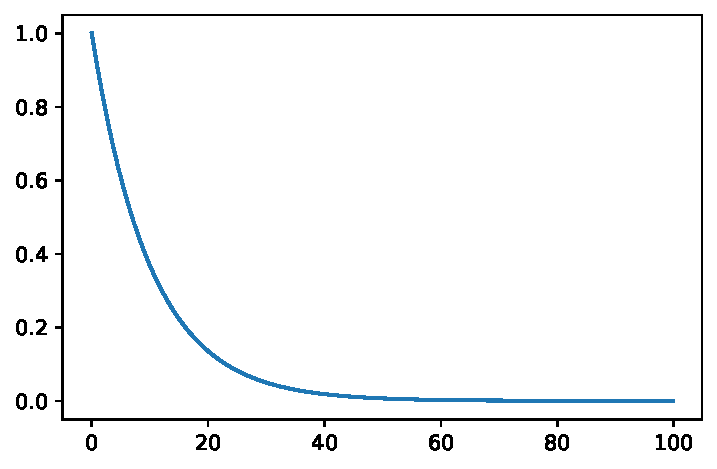
\includegraphics{./survival_files/figure-pdf/cell-2-output-1.pdf}

}

\end{figure}

\hypertarget{chapter-2---life-tables}{%
\section{Chapter 2 - Life Tables}\label{chapter-2---life-tables}}

See notes - Two example type to be practiced exhaustively (No loss and
loss to follow up)

Lifetables tabulate death rates over a period of time. They are useful
non-parametric summaries and help to inform which parametric models
might be sensible.

In the loss to follow up we assume in this course that:

\begin{itemize}
\tightlist
\item
  \(p_x\) and \(q_x\) are constant over a time period, this is
  reasonable if short
\item
  We assume those who withdraw have the same probability of dieing as
  those who don't
\item
  We assume withdrawls are evenly spaced through the year
\end{itemize}

TODO: Finalise life tables with method.

\hypertarget{chapter-2.4---kaplan-meier}{%
\section{Chapter 2.4 - Kaplan-Meier}\label{chapter-2.4---kaplan-meier}}

Life tables are just summaries. They result in a loss of alot of
information as the bin dates. Kaplan-Meir is more useful if you have
access to the raw data.

The full name of this chapter is the ``Kaplan-Meier Product Limit
Estimate of S(t)''

\begin{quote}
This can be practised endlessly using \texttt{survfit}
\end{quote}

\hypertarget{no-censoring}{%
\subsection{No Censoring}\label{no-censoring}}

Note - The somewhat obscure inclusion of at risk becomes clear when you
include censored values.

If there are \(n\) observed times to failures (\(t_i\)) we can order the
times (provided there are k distinct). So

\(t_1, t_2, ... t_n\) becomes \(t_{(1)} < t_{(2)} < ... < t_{(k)}\). If
\(d_i\) is the number of deaths at time \(t_{(i)}\) then :

\(\sum_{i=1}^k d_i = n\)

If we knwo this then we can estimate the CDF by:

\(\hat{F}(t) = \text{Proprtion of lifetimes that are} < t\)

So if we are given a time \(t\) to calculate we can use the following
equation to approximate:

\(\frac{1}{n} \sum^{s}_{i=1}d_i\) where \(t_s\leq t \leq t_{s+1}\)

So as \(\hat{S}(t) = 1 - \hat{F}(t)\) we can easily calc by

\(1 - \frac{1}{n} \sum^{s}_{i=1}d_i = \frac{n - \sum^{s}_{i=1}d_i }{n}\)

A useful trick however is to consider \(r_j\) those ``at risk'' (those
who are still alive) just before time \(t_j\). Just before \(t_j\) we
know that \(r_{j+1} = r_j - d_j\). In lay terms the number at risk next
is the number who were previoulsy at risk less those who just died.

By a telescoping series like effect it can be shown that (notice
trailing numerator cancel leading denominator)

\(\hat{S}(t) = \frac{n-d_1}{n} \times \frac{n-d_1 - d_2}{n - d_1} \times \frac{n-d_1 - d_2- d_3}{n - d_1 - d_2} \times ... \times \frac{n - d_1 - ... - d_s}{n - d_1 - ... - d_{s-1}}\)

At risk \(r\) can now be incorperated. as

\(\hat{S}(t) = (1 - \frac{d_1}{r_1}) \times (1 - \frac{d_2}{r_2}) \times ... \times (1 - \frac{d_s}{r_s})\)

Simuplifying by notation therefore:

\(\hat{S}(t) = \prod^s_{j=1}( 1 - \frac{d_j}{r_j})\) for
\(t_s\leq t \leq t_{s+1}\)

It must hold that \(s\geq 1\) and anything before then is assume to
equal 1. If everyone dies then the KP curve will go to zero.

\hypertarget{with-censoring}{%
\subsection{With Censoring}\label{with-censoring}}

Because we have included the at risk aspecty, censoring is treated in a
very similar way except the at risk aspect is modified.

To calculate those at risk just before time \(t\) we need to know who
was cencosred. We introduce an \(I_j\) term which is the number of
people censored in the time interval \(t_{j-1} \leq t \leq t_j\)

\(r_1 = n - I_1\)

More generally

\(r_j = r_{j-1} - d_{j-1} - I_j\)

\hypertarget{calculating-median-st-with-km}{%
\subsection{Calculating median S(t) with
KM}\label{calculating-median-st-with-km}}

The median survival time is the smallest value of time where the
survivor function takes a value of 0.5 or less.

So for instance in your Kaplan-Meier table you have a something like
this

\begin{longtable}[]{@{}ll@{}}
\toprule()
time & S(t) \\
\midrule()
\endhead
4 & 0.55 \\
8 & 0.47 \\
\bottomrule()
\end{longtable}

Then the median survival time is 8

\hypertarget{notes}{%
\subsection{Notes}\label{notes}}

\begin{itemize}
\tightlist
\item
  KM relies on short intervals for recording death, if not completely
  continuous. It will not work for things like lifetables
\item
  If uncencorsed \(I_j\) is always 0 so you get the same thing again
\item
  If the last observation(s) are censcored then the KM curve never
  reaches 0 but carries on forever. Obviously this isn't real and so
  becomes biased if the last observation(s) are censored.
\item
  Greenwoods provides a formula for sampling error
  \(var(\hat{S}(t)) = (\hat{S}(t))^2 \sum^s_{j=1} \frac{d_j}{r_j(r_j - d_j)}\)
  for \(t_s\leq t \leq t_{s+1}\)
\item
  Hazard can also be calculated as \(\hat{H}(t) = -log\hat{S}(t)\). A
  simplae approiximation for hazard can be shown to be
  \(H(t) \approx \sum_{j-1}^s\frac{d_j}{r_j}\)
\end{itemize}

\hypertarget{exam-method}{%
\subsection{Exam method}\label{exam-method}}

\begin{quote}
This can be practised endlessly using \texttt{survfit}
\end{quote}

TODO: COMPLETE THIS AFTER SIME PRACTICE

\begin{enumerate}
\def\labelenumi{\arabic{enumi})}
\tightlist
\item
  Create a j col from 0 \ldots. to number of unique death timestamp, 0
  is a unique time too.
\item
  List all unique deaths in \(t_{(j)}\) column. DO NOT INCLUDE CENSOR
  TIMES. 0 is a valid time.
\item
  Leave 0 row blank with exception of \hat{S(t)} column, set that to 1.
\item
  Make censor column (\(I_j\)) denotes all censored values in the
  preceding window.
\item
  create deaths column \(d_j\)
\item
  Create an at risk column. This is the most complicated,
  \(r_j = r_{j-1} - d_{j-1} - I_j\)
\item
  Calultate \(1 - \frac{d_j}{r_j}\)
\item
  \(\hat{S}(t)\) is the product of 7
\item
  Create a \(t\) column much like a CDF where \(0 \leq t < d_1\)
  (intervals are critical to marks/understanding)
\item
  first \(t_j\) to be less than 0.5 is the median!
\end{enumerate}

\begin{quote}
remember \(r_1 = n - I_1\)
\end{quote}

\begin{quote}
If in doubt think hard about \(\leq t <\) for placing deaths, logic. In
the notes we put it last, I think it should almost go first.
\end{quote}

\hypertarget{chapter-2.5---parametric}{%
\section{Chapter 2.5 - Parametric}\label{chapter-2.5---parametric}}

TODO : In this I largely gloss over the likelihood stuff. It feels
unlikely it will be examined and I will retun if time.

This chapter assumes an exponetial distribution \(T \sim Exp(\lambda)\)
is being used.

When doing likelihood for uncensored data you follwo the usual path of
finding the Likelihood by multiplying through, get log likelihood if
convinient and differentiating with respect to the paramater. So

\(L(\lambda ; t_1, t_2 ... t_n) = \prod^n_{i=1}f(t_i)\)

In the censored case however this becomes a little more complicated. You
cannot just multiply by the desnities as you do not know the density for
the censored values.

If we observed a death then \(f(t)\) contributes to the likelihood.
However if we do not observed the death \(t_i > c_i\) then we say that
we know they survived longer than some time so \(P(T > c_i) = S(c_i)\).
And this contributes to the likelihood.

By combining density and survivor functions and applying the indicator
0=censor, 1=death. The following form of the likelihood can be created:

\$L(\lambda) = \prod\_\{i=1\}\^{}n
f(t\_i)\^{}\{\delta\_i\}S(c\_i)\^{}\{1-\delta\_i\} = \$

\(L(\lambda) = \prod_{i=1}^n [\lambda e^{-\lambda t_i}]^{\delta_i}[e^{-\lambda c_i}]^{1-\delta_i}\)

It can then be shown that:

\(\hat{\lambda} = \frac{\sum^n_{i=1} \delta_i}{\sum^n_{i=1}(t_i\delta_i +(1-\delta_i)c_i)}\)

And

\(var(\hat{\lambda}) \approx \frac{\hat{\lambda}^2}{\sum^n_{i=1} \delta_i}\)

By asymptopic normality of the MLE the 95\% CI is
\(\hat{\lambda}\pm 1.96\sqrt{var(\hat{\lambda}}\)

For the exponential we calculate the mean by
\(\frac{1}{var(\hat{\lambda})}\) and the variance of this can be shown
to be

\(var(\hat{\mu}) = \frac{\hat{\mu}^2}{\sum_{i=1}^n \delta_i}\)

TODO: What is the value in learning equation 56/61 with exp denom. TODO:
RAndom censoring, log normal and others (2.5.6)

\hypertarget{using-r---exponetial}{%
\subsection{Using R - Exponetial}\label{using-r---exponetial}}

The exponetial model can be fitted in r with \texttt{survreg}, where
\texttt{dist=\textquotesingle{}exponential\textquotesingle{}}.

For the MLE of \(\hat{\lambda}\) you take \(exp(-\beta_0)\) assuming no
covariates eg \texttt{time\ \textasciitilde{}\ 1}. The easiest way to
get the CI is to apply +/- 1.96 standard error to beta pre exponent.
This will give some minor disagreement though to the division by death
count method.

\begin{quote}
\(\hat{\lambda} = exp(-\hat{\beta_0} \pm 1.96\times se(\hat{\beta_0}))\)
\end{quote}

\hypertarget{using-r---weibull}{%
\subsection{Using R - Weibull}\label{using-r---weibull}}

Under the weibull again
\(\hat{\lambda} = exp(-\hat{\beta_0} \pm 1.96\times se(\hat{\beta_0}))\)
and \(\hat{\gamma} = \frac{1}{\text{scale}}\)

The weibull is summarised in our work as
\(T \sim Weibull(\lambda, \gamma)\)

When \(\gamma = 1\) we are left with the exponential distribution.

\hypertarget{workflow-1}{%
\subsection{Workflow:}\label{workflow-1}}

\begin{enumerate}
\def\labelenumi{\arabic{enumi}.}
\tightlist
\item
  fit a kaplan-meier. Is the decay expoenntial? then exp could make
  sense
\end{enumerate}

\hypertarget{chapter-3---two-sample}{%
\section{Chapter 3 - Two Sample}\label{chapter-3---two-sample}}

Kaplan-Meier is just a visual aid, we need to look at tests

\hypertarget{log-rank-test}{%
\subsection{Log Rank Test}\label{log-rank-test}}

Non-parametric.

\[ H_0 : S_1(t) = S_2(t)\]

\[ H_A : S_1(t) \neq S_2(t)\]

\(H_A\) is for some \(t\)

Steps:

\begin{enumerate}
\def\labelenumi{\arabic{enumi})}
\tightlist
\item
  Create a table
\item
  create an \(i\) column for 1,2,..n
\item
  create a \(t_i\) column and list all the times of deaths only
\item
  Create an \(r_{1,i}\) and \(r_{2,i}\) for at risk (At risk for a time
  includes those who died at that time and all future censorees)
\item
  Sum \(r_{1,i}\) and \(r_{2,i}\) to get \(r_i\) (row wise)
\item
  Create an \(d_{1,i}\) and \(d_{2,i}\) for death counts at the times
\item
  Sum the deaths to get \(d_i\)
\item
  Sum down death column to get observed \(O_1\) and \(O_2\)
\item
  Calc \(e_{1,i} = (\frac{r_{1,i}}{r_i})d_i\) and \(e_{2,i}\)
\item
  Sum the \(e_{1,i}\) and \(e_{2,i}\) to get \(E_1\) and \(E_2\)
\item
  Calculate using below equation
\end{enumerate}

\[ LR = \frac{(O_1 - E_1)^2}{E_1} + \frac{(O_2 - E_2)^2}{E_2} \sim \chi^2_{1}\]

To perform the logrank in r perform the following
\texttt{survdiff(formula\ =\ \textquotesingle{}time\ \textasciitilde{}\ treatment\textquotesingle{})}

\hypertarget{parametric}{%
\subsection{Parametric}\label{parametric}}

There are two types of parametric methods of interest MLE test and
Likelihood ratio

\hypertarget{mle-test}{%
\subsection{MLE Test}\label{mle-test}}

Effectively looks at the paramters as normally distributed (though any
test, distribution is applicable). Then performs standard tests upon
them. So in the case of lambda, given it is normally distributed as an
estimator.

\(\frac{\hat{\lambda}_1 - \hat{\lambda}_2}{\sqrt{\frac{\hat{\lambda}_1^2}{\Delta_1}-\frac{\hat{\lambda}_2^2}{\Delta_2}}} \sim N(0,1)\)

Here \(\Delta\) is the number of deaths and \(\hat{\lambda}\) is the
number of deaths over total time (death and censor).

\hypertarget{likelihood-ratio}{%
\subsection{Likelihood Ratio}\label{likelihood-ratio}}

In formula sheet

TODO: run through the proof

\hypertarget{survreg}{%
\subsection{\texorpdfstring{\texttt{Survreg}}{Survreg}}\label{survreg}}

From survreg we can use the output of a two factor analysis to easily do
a MLE test by taking the parameter and covariance matrix.

For LRT look at the following line near the bottom for the p-value.

Chisq=1.2 on 1 degrees of freedom , p=0.27

\bookmarksetup{startatroot}

\hypertarget{linear-models}{%
\chapter{Linear Models}\label{linear-models}}

\hypertarget{intro}{%
\section{Intro}\label{intro}}

Categorical variables are called factors, they may be binary or have
levels

y may be reffered to as dependnent or response variable(s)

x may be called independent , explanatory, predictor variables.

We use \(n\) to denote observations

We use \(r\) for the number of explanatory variables.

A model might look like

\(y_i = \beta_0 + \beta_1x_{i1} + ... \beta_{ir} + \epsilon_i\)

The \(\beta_0 + \beta_1x_{i1} + ... \beta_{ir}\) is reffered to as the
linear predictor. Epsilon is the random error.

When r=2 we fit a plane! Then hyper-planes in higher dimensions.

Remember a linear model is linear in the parameters (betas), it is
allowed to include logs, quadratics.

It is easier to work in matrix notation. Parameter vector:

\(\boldsymbol{\beta} = (\beta_0, \beta_1, ...)^T\)

The \(\boldsymbol{x} = (x_1, x_2...)^T\) is combined with a vector of
ones to create the design matrix \(\boldsymbol{X}\).

This combined creates

\(\boldsymbol{y} = \boldsymbol{X} \boldsymbol{\beta}+ \boldsymbol{\epsilon}\)

\(\boldsymbol{X}\) has the shape \(n \times p\)

\(\boldsymbol{\beta}\) has the shape \(p \times 1\)

In linear modelling we assume that the \(\epsilon\):

\begin{itemize}
\tightlist
\item
  Is a MV Norm
\item
  0 Mean
\item
  Independent
\item
  Common variance \(\sigma^2\) (homoscedasticity)
\end{itemize}

So :

\(\epsilon \sim N_n(0, \sigma^2 I_n)\)

And if \(y = X\beta + \epsilon\) then we can say by linear
transformation that

\(y \sim N_n(X\beta, \sigma^2 I_n)\)

In this course:

\begin{itemize}
\tightlist
\item
  Explanatory - the base \(x\) variable, from the data
\item
  Regressor - The constant, the \$\beta x \$ and any function or
  transform of \(x\) with a coefficient.
\end{itemize}

So \(y = \beta_0 + \beta_1 x \beta_2 x^2\) has a single explantory
variable, but 3 regressors.

\hypertarget{chaprter-2---fit-estimate-and-residuals}{%
\section{Chaprter 2 - Fit, estimate and
residuals}\label{chaprter-2---fit-estimate-and-residuals}}

Once fitted the the difference between the observed actual and fitted
values (\(x_i^T\hat{\beta}\)) is the residual. The vector of residuals
therefore can be calced as:

\(e = y - X\hat{\beta}\)

The \textbf{sum of squared of the residuals} or \textbf{residual su of
squares} (\(S_r\)) is very important

\(S_r = S(\hat{\boldsymbol{\beta}}) = \sum_{i=1}^n e_i^2 =\textbf{e}^T\textbf{e} = (y - X\hat{\beta})^T(y - X\hat{\beta})\)

\begin{quote}
In linalg rememeber that \(x^Tx\) of a columnar vector is equivalent to
\(\sum x^2_i\)
\end{quote}

This concept is very useful in linear modelling because through the
MVNorm we can show that:

\(L(\beta, \sigma^2 ; y) = f(y|\beta. \sigma^2) \propto \sigma^{-n}\exp(- \frac{1}{2\sigma^2}(y - X\hat{\beta})^T(y - X\hat{\beta}))\)

A key part of this derivation is that \(|\sigma^2I_n| = (\sigma^2)^n\).
The log likelihood can be shown to be

\(\ell(\beta, \sigma^2;y) = -nlog(\sigma) - \frac{1}{2\sigma^2}(y - X\hat{\beta})^T(y - X\hat{\beta}) + c\)

To maximise likelihood with respect to \(\beta\) therefore we should be
looking to minimise \(S_r\). Minimising this is the \textbf{least
squares} method, which both mathematically and intuitively makes sense.
There is an important consequence!

\begin{quote}
Assuming X has rank p, the least squares estimator of \(\beta\) is
\(\hat{\beta} = (X^TX)^{-1}X^Ty\)
\end{quote}

When finding the MLE of \(\sigma^2\) we find \(\frac{S_r}{n}\), however
this is a biased estimator and instead we use \(\frac{S_r}{n-p}\)

\hypertarget{estimator-mean-and-variance}{%
\subsection{Estimator mean and
variance}\label{estimator-mean-and-variance}}

Given \(y \sim N_n(X\beta, \sigma^2I_n)\)

Uisng this we can show that \(\hat{\beta}\) is an unbiased estimator

\(E(\hat{\beta}) = E((X^TX)^{-1}X^Ty)\) where \(E(y) = X\beta\) so

\(E((X^TX)^{-1}X^TX\beta)\) , the \(X^TX\) terms cancel by inverse
leaving \(\beta\)

Furthermore \(Var(\hat{\beta})\) can be calculated:

\(Var(\hat{\beta}) = Var((X^TX)^{-1}X^Ty)\) where
\(Var(y) = \sigma^2I_n\)

Recall that given a non-stochastic matrix \(A\), and stochastic y, then
\(Var(Ay) = A Var(y) A^T\). From matrix laws too \((AB)^T = B^TA^T\) and
\((A^{-1})^T = (A^T)^{-1}\)

\(Var(\hat{\beta}) = Var((X^TX)^{-1}X^Ty) = (X^TX)^{-1}X^T Var(y)((X^TX)^{-1}X^T)^T\)

\(= (X^TX)^{-1}X^T Var(y) X((X^TX)^{-1})^T = (X^TX)^{-1}X^T Var(y) X((X^TX)^T)^{-1})\)

\(= (X^TX)^{-1}X^T Var(y) X(X^TX)^{-1}\)

\(= (X^TX)^{-1}X^T \sigma^2 I_n X(X^TX)^{-1}\)

\(= \sigma^2 (X^TX)^{-1}X^TX(X^TX)^{-1} = \sigma^2 (X^TX)^{-1}\)

\begin{quote}
\(\hat{\beta} = N_p(\beta, \sigma^2 (X^TX)^{-1})\)
\end{quote}

\hypertarget{error-variance-estimate}{%
\subsection{Error variance estimate}\label{error-variance-estimate}}

\(e = y-X\beta = y - X(X^TX)^{-1}X^Ty\), the \(y\) can be factorised out
to give

\(e = My\), where \(M = I_n - X(X^TX)^{-1}X^T\)

If \(E(e) = E(My) = ME(y) = MX\beta\)

\(MX = (I_n - X(X^TX)^{-1}X^T)X = X - X(X^TX)^{-1}X^TX = 0\)

So \(MX = 0\) therefore \(E(e) = 0\) . M is also \textbf{idempotent},
which means \(M^2 = M\). idempotent matrices (except \(I_N\)) are always
singular.

Another important result of M is that:

\(Var(e) = Var(My) = MVar(y)M^T = M\sigma^2I_nM =\sigma^2M^2 = \sigma^2M\)

So \(M\) is related to the variance-covariance matrix of the residuals.

\begin{quote}
The variance of an individual residual is \(\sigma^2\) times the
corresponding diagonal of \(M\)
\end{quote}

It can be shown (using trace and rank rules) that:

\(\hat{\sigma}^2 = \frac{1}{n-p}\sum^n_{i=1}e_i^2 = \frac{1}{n-p}S_r\)

The square root of this is the \textbf{residual standard error}, this is
given in the r output.

It can also be shown by probability theory that a MVNorm with covariance
matrix \(M\), that \(\frac{S_r}{\sigma^2} \sim \chi^2_{n-p}\)

\hypertarget{covariance}{%
\subsection{\texorpdfstring{\hat{\beta}
covariance}{ covariance}}\label{covariance}}

Rememeber that:

\(corr(\beta_0, \beta_1) = \frac{Cov(\hat{\beta_0},\hat{\beta_1})}{se(\hat{\beta_0}) \times se(\hat{\beta_1)}}\)

\hypertarget{model-fit-coefficient-of-determination-r2}{%
\section{\texorpdfstring{Model Fit : Coefficient of determination
\(R^2\)}{Model Fit : Coefficient of determination R\^{}2}}\label{model-fit-coefficient-of-determination-r2}}

\(S_r\) can be thought of as a measure of fit. However it will vary
depending magnitudes of the variables, so cannot be compared directly
between different problems. To enable better comparison we standardise
with \(S_{yy}\) (Total sum of squares), \(R^2\) may also be called the
coefficient of determination.

\(R^2 = \frac{S_{yy} - S_r}{S_{yy}}\) where
\(S_{yy} = (y-\bar{y})^T(y-\bar{y}) = y^Ty - n\bar{y}^2\)

In simpler terms:

\begin{itemize}
\tightlist
\item
  \(R^2\) is the proportion of the total sum of squares that the model
  explains
\item
  Whilst \(S_r\) is the explained part of \(S_{yy}\)
\end{itemize}

\(S_{yy}\) may also be written as \(SS_{Total}\)

Relying on \(R^2\) alone for model comparison is not sensible as it will
always increase when parameters are added. The use of adjusted \(R^2\)
is preffereable as it takes into account the number of parameters.

\(R^2(adj) = 1 - \frac{S_r/(n-p)}{S_{yy}/(n-1)}\)

\hypertarget{confidence-and-prediction-intervals}{%
\section{Confidence and Prediction
Intervals}\label{confidence-and-prediction-intervals}}

\hypertarget{chapter-4---hypothesis-testing}{%
\section{Chapter 4 - Hypothesis
testing}\label{chapter-4---hypothesis-testing}}

The most natural and simple hypothesis is whether a given \(\beta\) is
equal to 0. It has no effect on the model.

However there might be more general null hypothesis. Eg:

\begin{itemize}
\tightlist
\item
  \(\beta_1 = \beta_2 = \beta_3 = 0\)
\item
  \(\beta_1 = \beta_2\)
\end{itemize}

To cover all bases (for linear hypothesis) however we can say:

\(H_0 : \boldsymbol{C\beta} = c\)

\(H_A : \boldsymbol{C\beta} \neq c\) (At least one is not equal.)

C is \(q \times p\) and c is \(q \times 1\) of known constants. C has
rank q, so full rank. So at each row of C and c we are asserting some
hypothesis that the linear combination of C is equal to c.~With this
framework it is not possible to specify one-sided tests, though this is
rarely of interest.

\hypertarget{some-eamples-of-c-and-c}{%
\subsection{Some eamples of C and c}\label{some-eamples-of-c-and-c}}

\(H_0 : \beta_1 = 1, \beta_2=2\)

\(C = \begin{pmatrix} 0 & 1 & 0\\ 0 & 0 & 1 \end{pmatrix} = \begin{pmatrix} 1 \\ 2 \end{pmatrix}\)

\hfill\break

\(H_0 : \beta_1 = \beta_2 = 0\)

\(C = \begin{pmatrix} 0 & 1 & 0\\ 0 & 0 & 1 \end{pmatrix} = \begin{pmatrix} 0 \\ 0 \end{pmatrix}\)

\hfill\break

\(H_0 : \beta_2 = 0\)

\(C = \begin{pmatrix} 0 & 0 & 1 \end{pmatrix} = \begin{pmatrix} 0 \end{pmatrix}\)

\hfill\break

\(H_0 : \beta_2 = 3\)

\(C = \begin{pmatrix} 0 & 0 & 1 \end{pmatrix} = \begin{pmatrix} 3 \end{pmatrix}\)

\hfill\break

\(H_0 : \beta_1 = \beta_2\) Which is equivalent to
\(H_0 : \beta_1 - \beta_2 = 0\)

\(C = \begin{pmatrix} 0 & 1 & -1 \end{pmatrix} = \begin{pmatrix} 0 \end{pmatrix}\)

\hypertarget{test-stat-q-1}{%
\subsection{Test Stat q \textgreater{} 1}\label{test-stat-q-1}}

\begin{equation}\protect\hypertarget{eq-f-test}{}{\frac{(C \hat{\beta} -c )^T(C(X^TX)^{-1}C^T)^{-1}(C \hat{\beta} -c )}{q\hat{\sigma}^2} \sim F_{q, n-p}}\label{eq-f-test}\end{equation}

Note : This is a one-sided test so \(1-\alpha\) (0.95) not
\(1-\alpha / 2\) (0.975, 95\% CI). This is due to square terms.

\hypertarget{test-stat-q-1-1}{%
\subsection{Test Stat q = 1}\label{test-stat-q-1-1}}

When there is only one test eg. \(\beta_1=0\) then the abiove equation
can be simplified to a t-test. This becomes:

\(\frac{\hat{\beta}_i - c_i}{\hat{\sigma} \sqrt{g_{ii}}} \sim t_{n-p}\)

Where \(G = (X^TX)^{-1}\) and \(g_{ii}\) is the \emph{i}-th diagonal
term.

\hypertarget{some-notes}{%
\subsection{Some notes}\label{some-notes}}

The r \texttt{summary} will tell you \(\hat{\sigma}\) through the
``Residual Standard Error'' line

The F-Statistic in \texttt{summary} is testing whether all coefficients
other than intercept are 0

Pay little attention to tests of the individual coefficients if doing
multi coeefficent tests. Significance can easily flip between all and
individuals. Even if all are indicating p\textgreater0.05 and test says
p\textgreater0.05.

\hypertarget{nested-models}{%
\subsection{Nested models}\label{nested-models}}

By nested models we mean comparing one model to another, where one of
them contains a subset of the other. It is usually used to determine
whether there is value in including the term in the term(s) in the
model.

We are trying to trade off increasing regression sum of squares vs
excluding the term. So there is value in verifying whether something
should be included.

An example is:

\(y= \beta_0 + \beta_1x_1\) vs \(y= \beta_0 + \beta_1x_1 + \beta_2 x^2\)

So does \(\beta_2 = 0\)?

For nested models we use a similar framework to before but modify the
\(\beta\) vector. The C matrix becomes a 0 matrix with the indentity
matrix appended to the right where the \(I_n\) has an n of \(p_f - p_r\)
where \(p_f\) is parameter in the full model and \(p_r\) is the number
of params in the reduced model.

In \(\boldsymbol{\beta}\) we have a stack of vectors
\((\boldsymbol{\beta}_1, \boldsymbol{\beta}_2)^T\). Where
\((\boldsymbol{\beta}_1\) is a \(p_r \times 1\) and
\((\boldsymbol{\beta}_2\) is a \((p_f - p_r) \times 1\).

Element order is arbituary provided that we are consistent between all
matrices and vectors.

A useful summary is via ANOVA tables where:

\begin{longtable}[]{@{}
  >{\raggedright\arraybackslash}p{(\columnwidth - 8\tabcolsep) * \real{0.2247}}
  >{\raggedright\arraybackslash}p{(\columnwidth - 8\tabcolsep) * \real{0.2360}}
  >{\raggedright\arraybackslash}p{(\columnwidth - 8\tabcolsep) * \real{0.0562}}
  >{\raggedright\arraybackslash}p{(\columnwidth - 8\tabcolsep) * \real{0.2022}}
  >{\raggedright\arraybackslash}p{(\columnwidth - 8\tabcolsep) * \real{0.2809}}@{}}
\toprule()
\begin{minipage}[b]{\linewidth}\raggedright
Source of Variation
\end{minipage} & \begin{minipage}[b]{\linewidth}\raggedright
Sum of Squares (SS)
\end{minipage} & \begin{minipage}[b]{\linewidth}\raggedright
DoF
\end{minipage} & \begin{minipage}[b]{\linewidth}\raggedright
Mean Square (MS)
\end{minipage} & \begin{minipage}[b]{\linewidth}\raggedright
Mean Square Ratio (MSR)
\end{minipage} \\
\midrule()
\endhead
Due to \(X_1\) is \(\beta_2\) = 0 & \(S_1\) & \(p_r\) & \(S_1 / p_r\) &
\(F_1\) \\
Due to \(X_2\) only & \(S_2\) & \(p_f - p_r\) & \(S_2 /(p_f - p_r)\) &
\(F_2\) \\
Residual & \(S_r\) & \(n -p_f\) & \(\hat{\sigma}^2\) & \(F_2\) \\
Total & \(y^Ty\) & n & & \\
\bottomrule()
\end{longtable}

The MSR are calculated by dividing the variance of each model by the
product of the Dof and residuals so:

\(F_2 = \frac{S_2}{(p_f-p_r)\hat{\sigma}^2}\)

\(F_1 = \frac{S_1}{p_r\hat{\sigma}^2}\)

We typically work through these tests in sequence, firstly test 2 then
test 1.

The initial test on \(F_2\) is just the test in
Equation~\ref{eq-f-test}. Where the null is \(\beta_2 = 0\) and the null
dist is \(F_{p_f-p_r, n-p_f}\) (remember it's one sided) and we test if
\(F_2 >F_{p_f-p_r, n-p_f}\). \(F_2\) can also be calculated from
residual sum of squares of models (RSS,, which can be obtained from
ANOVA summary in R).

\begin{equation}\protect\hypertarget{eq-exam-f}{}{F_2 = \frac{(RRS_r - RSS_f) / (p_f - p_r)}{(RSS_f)/(n-p_f)}}\label{eq-exam-f}\end{equation}

After \(\beta_2\) we test the hypothesis that \(\beta_1=0\) given we
know \(\beta_1\) is 0, or \(\boldsymbol{\beta}=\textbf{0}\) (this is a
little handwavy as the test doesn't poove the null, but it is accepted
convention).

We test \(F_1 > F_{p_r, n-p_f}\)

\hypertarget{minimal-model}{%
\subsection{Minimal model}\label{minimal-model}}

A special test based on the previous section. If we set \(c=0\) and
\(C=I\) we would test that every single coefficient is equal to zero.
This basically tests that y is 0 and constant irrespetive of the
variables. What we really want to test howeveris that y has a floating
mean, but is constant.

Therefore we test that the regressors only are zero by saying
\(\beta_1 = \beta_0\) and that the \(\beta_2\) is just all the
regressors, making a p-1 length. The \(\beta_0\) model is called the
minimal or null model, with a mean of \(\beta_0\) and variance of
\(\sigma^2\). As we don't really care if \(beta_0\) is 0 or not we
exclude it from the ANOVA tables.

TODO: read this
https://stats.stackexchange.com/questions/256726/linear-regression-what-does-the-f-statistic-r-squared-and-residual-standard-err

So in this model \(p_r=1\) and \(p_f = p-1\)

It can be show (see notes p29) that:

\begin{longtable}[]{@{}
  >{\raggedright\arraybackslash}p{(\columnwidth - 8\tabcolsep) * \real{0.2247}}
  >{\raggedright\arraybackslash}p{(\columnwidth - 8\tabcolsep) * \real{0.2360}}
  >{\raggedright\arraybackslash}p{(\columnwidth - 8\tabcolsep) * \real{0.0562}}
  >{\raggedright\arraybackslash}p{(\columnwidth - 8\tabcolsep) * \real{0.2022}}
  >{\raggedright\arraybackslash}p{(\columnwidth - 8\tabcolsep) * \real{0.2809}}@{}}
\toprule()
\begin{minipage}[b]{\linewidth}\raggedright
Source of Variation
\end{minipage} & \begin{minipage}[b]{\linewidth}\raggedright
Sum of Squares (SS)
\end{minipage} & \begin{minipage}[b]{\linewidth}\raggedright
DoF
\end{minipage} & \begin{minipage}[b]{\linewidth}\raggedright
Mean Square (MS)
\end{minipage} & \begin{minipage}[b]{\linewidth}\raggedright
Mean Square Ratio (MSR)
\end{minipage} \\
\midrule()
\endhead
Due to regressors & \(S_2 = \hat{\beta}^TX^TX\hat{\beta} - n \bar{y}^2\)
& \(p-1\) & \(S_2 / (p-1)\) & \(F\) \\
Residual & \(S_r = y^Ty -\hat{\beta}^TX^TX\hat{\beta}\) & \(n -p\) &
\(\hat{\sigma}^2\) & \\
Total & \(S_{yy} =y^Ty - n\bar{y}^2\) & n-1 & & \\
\bottomrule()
\end{longtable}

So \(F = \frac{S_2}{(p-1)\hat{\sigma}^2}\) where null is
\(F_{p-1, n-p}\)

TODO: what are they talking about top of p30

\hypertarget{anova---application-in-r}{%
\subsection{ANOVA - Application in R}\label{anova---application-in-r}}

\begin{quote}
This is highly likley to be examined
\end{quote}

With r you have two choices for ANOVA one where you enter each model
seperately where one model is the baseline and the other is more complex
so :

\begin{itemize}
\tightlist
\item
  \(y = \beta_0 + \beta_1x_1\) (mdl\_1)
\item
  \(y = \beta_0 + \beta_1x_1 + \beta_2x_1^2\) (mdl\_2)
\end{itemize}

so \texttt{anova(mdl\_1,\ mdl\_2)} or you simply run
\texttt{anova(mdl\_2)}.

In the first option it automatically detects the extra terms and assigns
those to \(\beta_2\) and then \(H_0: \beta_2 = 0\) is assessed. Values
from the summary of this can readily be placed into
Equation~\ref{eq-exam-f}.

TODO : Down from the blue arrow

\hypertarget{chapter-5}{%
\section{Chapter 5}\label{chapter-5}}

Remember:

\(\epsilon_i = y_i - \textbf{x}_i^T\boldsymbol{\beta}\)

We assume that \(\epsilon_i\) is:

\begin{itemize}
\tightlist
\item
  0 mean, there is no systematic error from
  \(\textbf{X}\boldsymbol{\beta}\)
\item
  Independent
\item
  Common variance - homoscedasticity
\item
  Normaly distributed
\end{itemize}

We check these through residuals (the estimate of the error based on
fitted model). If the model were to be correct they would be normally
distributed, however they are not independent or with common variance.
Unequal variances can be corrected for by standardised residuals:

\(s_i \frac{e_i}{\sqrt{\hat{\text{Var}}(e_i)}} \sim t_{n-p}\) where
\(\hat{\text{Var}}(e_i)\) is the estimate of variance

\begin{quote}
observed residuals are not independent and do not have equal variances
\end{quote}

\hypertarget{q-q-plot}{%
\subsection{q-q plot}\label{q-q-plot}}

Plots quantiles of observed vs expected and you should get a straight
line, you may plot:

\begin{itemize}
\tightlist
\item
  Standard Normal against observed data
\item
  Normal with mean and variance of observed against observed data
\item
  Standardised residual
\end{itemize}

You should see a straight line of plots if the fit is appropriate. If:

\begin{itemize}
\tightlist
\item
  The plot is bowed there is skew
\item
  Down left/Up right = heavier tails
\end{itemize}

Histograms should be avoided if the dataset is small.

\hypertarget{homoscedasticity}{%
\subsection{Homoscedasticity}\label{homoscedasticity}}

Plot a scatter graph of residual against the fitted value (y predicted).
This should be a uniform band. Typically issues arise where the results
fan outwards to the larger values

\hypertarget{independence}{%
\subsection{Independence}\label{independence}}

Typically we plot the residual in observed order, through an ``index
plot''. The order is based on SME knowledge (time, distance,etc). We are
looking for trends, closely linked order points, etc.

\hypertarget{formal-testing}{%
\subsection{Formal testing}\label{formal-testing}}

We can formally test whether the residuals contain outliers by
standardising the residuals and looking for points. If the standardised
residuals (\(s_i\)) are t distributed we can assess how ``likely'' they
are by assessing the quantiles.

However if we were to do this for every point we are multiple testing
and so a corrrection to the cut off should be applied.Formally:

\(|s_i| > t_{n - p, 1-\alpha/2}\)

Instead of the bonferonni test we could use the Šidák correction which
is:

\begin{quote}
\(\alpha^* = 1 - (1-\alpha)^{1/n}\), where \(\alpha^*\) is the adjusted
stat.
\end{quote}

\hypertarget{chapter-6---interactions-and-factors}{%
\section{Chapter 6 - Interactions and
Factors}\label{chapter-6---interactions-and-factors}}

We include factors through the use of dummy or indicator variables.
Where the are two levels this will simply be a 0/1. For more than one
catergory, one-hot encoding will be used.

With dummy variables you have to be very careful not to over
parameterise the model.

You cannot have a model constant and a constant for each factor this is
overparameterisation and leads to multicolinearity. A matrix is not full
rank when there are linear combinations. Therefore \(X^TX\) is no longer
invertable (singular). Therefore we cannot calculate \(\hat{\beta}\)
through \((X^TX)^{-1}X^T y\).

The solution is to move to the following representation:

\(y_{ij} = \mu + \alpha_i + \epsilon_{ij}\)

This can be implement one of two ways

\hypertarget{level-one-zero-constraint}{%
\subsubsection{Level One Zero
Constraint}\label{level-one-zero-constraint}}

Also known as \textbf{corner points constraints}. Essentially the first
catergorcial variable is used for \(\mu\) and the first \(\alpha_1\) is
set to zero removing it from the model and the design matrix.

All other \(\alpha_i\) i=(2,3,\ldots k) are therefore deviations from
the mean (\(\mu\)) and hence how the mean of y changes as we move
between factors.

\texttt{options(contrast=c(factor=\ ...,\ ordered\ =...))} will
implement this in R

\hypertarget{sum-to-zero}{%
\subsubsection{Sum to Zero}\label{sum-to-zero}}

An alternative where all of the \(\alpha\) values are designed to sum to
zero. In a one factor model the \(\mu\) is therefore the overall mean,
while \(\alpha\) is the factor group means deviation from the this.

This method does remove a parameter, it is achievd by accounting for the
sum of all alphas from 1 to k-1 and setting k equal to the negative sum
of these so they cancel. X therefore loses it's \(\alpha_k\) column, but
also modifies all other \(alpha_i\) columns where the \textbf{row} is
i=k

TODO: This is a bit lost on me, see p46/47

\hypertarget{two-way-factors}{%
\subsection{Two way factors}\label{two-way-factors}}

In the two way factor you have rows and columns. In the corner point
constraint the mean is set by the top left mean. Then an \alpha\$
deviation is reported for 2,3,\ldots k rows and a \(\beta\) for
2,3,\ldots k columns.

\hypertarget{interactions}{%
\subsection{Interactions}\label{interactions}}

Interactions are non additive effects of one variable on anaother, this
is most commonly achieved through multiplication. These terms can be
tested for significance using \texttt{summary} or nested comparisions
conducted with \texttt{anova}. Care must be taken with factors as it is
easy to get high number of combinations, inflate \(R^2\) through
overfitting or get muktiplicity problems with signiificance.

\bookmarksetup{startatroot}

\hypertarget{survival-1}{%
\chapter{Survival}\label{survival-1}}

The first thing we are interested in is setting a baseline for the
explanatory variables \(\textbf{x}\). Where \(\textbf{x}\) becomes the
zero vector \(\textbf{0}\). Eg. \(\textbf{x} = (0,0,0...,0)\).

It is very common for age to be standardised around some age of
interest. Eg 50, so all ages would be given as 5, -10, etc which equates
to 55 and 40.

The two common methods are :

\begin{itemize}
\tightlist
\item
  Accelarated Failure Time (AFT)
\item
  Proportional Hazards (PH)
\end{itemize}

\hypertarget{aft}{%
\section{AFT}\label{aft}}

\hypertarget{two-group-example}{%
\subsection{Two Group Example}\label{two-group-example}}

In the simplests case we model survival times \(T\) as a random
variable. But with two groups we want to model them both as seperate
RVs. Where the baseline RV is \(T_0\) and the treatment (or other
covariate) is given by \(T_1\). As we now have times we can therefore
model survivor functions \(S\). However in AFTs we don't want \(S_0\)
and \(S_1\) we want a single survivor function that is scaled.

We therefore look to the following:

\(\text{Group 0 :   } S(t ; x_i=0) = P(T_0>t) = S_0(t))\)
\(\text{Group 1 :   } S(t ; x_i=1) = P(T_1>t) = P(\frac{T_0}{\psi}> t) = P(T_0>\psi t) = S_0(\psi t))\)

So \(\psi\) ``accelrates time'' and hence AFT and so the RVs are related
by \(T_1 = \frac{T_0}{\psi}\) and so \(S_1(t) = S_0(\psi t)\).

Thinking back to graphing, any multiplier of a function value is a
stretch in x, whose magnitude is the reciprical. So a \(\psi >1\) will
shrink survival time by \(\frac{1}{\psi}\) and a \(\psi <1\) will extend
survival time.

So \(\psi >1\) accelrates time for the patient (so they are more likely
to die faster). Less than one Deaccelerates!

\begin{quote}
Scale factor is \(\frac{1}{\psi}\) , less than 1 means better survival
times for the patient
\end{quote}

So \(\psi\) is a function of \(\textbf{x}\), all of our covariates,
which determine the ``acceleration''

\hypertarget{generalising-to-two-groups}{%
\subsection{Generalising to two
groups}\label{generalising-to-two-groups}}

Instead of now having a \(\psi\) to turn on and off we now require
\(\psi(\textbf{x})\) so that we can create a scaling factor for each
individual. We therefore assume that (Where \(S_0\) is \(S(t)\) at the
baseline consitions where \(\textbf{x} = \textbf{0}\)):

\(S(t;\textbf{x}) = S_0(t\psi(\textbf{x}))\)

From this it can be shown that the following are true:

\(f(t;\textbf{x}) = f_0(t\psi(\textbf{x}))\psi(\textbf{x})\)

\(h(t;\textbf{x}) = h_0(t\psi(\textbf{x}))\psi(\textbf{x})\)

This can be derived by showing that that \(t\) being multiplie by
\(\psi\) and has \(S_0\) applied to it as a function. We know the
relationship between the survival function and the density fuinction.
\(S(t) = 1- F(t)\) differentiatiing we get negative density function. A
function of a function, means that we need to use the chain rul and
therefore gets the above. From the desnity we can get the hazard. TODO :
Write out derivation. More details can be found at 25mins, 8/12.

So again: \(T = \frac{T_0}{\psi(\textbf{x})}\)

We are yet to define \(\psi(\textbf{x})\) but tow conditions must be
met:

\begin{itemize}
\tightlist
\item
  \(\psi(\textbf{x})\geq 0\), so cannot have a negative time
\item
  \(\psi(\textbf{0}) = 1\), so that the basline has no strethcing
  effects.
\end{itemize}

From this a naturual choice is (it could be any functiion though):

\({\psi(\textbf{x})} = \exp(-\beta'\textbf{x})\)

This gives us our parameters, but excludes the intercept terms.
Recalling \(T = \frac{T_0}{\psi(\textbf{x})}\) then

\(E[T] = \exp(\beta'\textbf{x})E[T_0]\)

If \(\beta_i x_i\) is positive then the expected survival time increases
(good fro patient)

\hypertarget{exponetial-case}{%
\subsection{Exponetial Case}\label{exponetial-case}}

Using the above we can therefore start to create an exponential AFT. We
already know that for the exponential distribution:

\begin{longtable}[]{@{}
  >{\raggedright\arraybackslash}p{(\columnwidth - 4\tabcolsep) * \real{0.3571}}
  >{\raggedright\arraybackslash}p{(\columnwidth - 4\tabcolsep) * \real{0.3571}}
  >{\raggedright\arraybackslash}p{(\columnwidth - 4\tabcolsep) * \real{0.2857}}@{}}
\toprule()
\begin{minipage}[b]{\linewidth}\raggedright
Property
\end{minipage} & \begin{minipage}[b]{\linewidth}\raggedright
equation
\end{minipage} & \begin{minipage}[b]{\linewidth}\raggedright
AFT
\end{minipage} \\
\midrule()
\endhead
\(S(t)_0\) & \(e^{-\lambda t}\) &
\(S(t;\textbf{x}) = \exp(-\lambda t e^{-\beta'\textbf{x}})\) \\
\(h(t)_0\) & \(\lambda\) & \(\lambda e^{-\beta'\textbf{x}}\) \\
\(f(t)_0\) & \(\lambda e^{-\lambda t}\) &
\(\lambda e^{-\beta'\textbf{x}} \exp(-\lambda t e^{-\beta'\textbf{x}})\) \\
\bottomrule()
\end{longtable}

So if \(\textbf{x}_i\) is a p dimensional vector of explanatory
variables then we ca n by MLE find p+1 parameters
\((\lambda, \beta_1, \beta_2...\beta_p)\).

MLE is found by usual method, get derivative, set to 0, solve
iteratively. \(\hat{\lambda}\) and \(\hat{\beta}\) are found any by the
asymptopic properties of the MLE we know that:

\(\hat{\lambda} \sim N(\lambda, \text{Var}(\hat{\lambda}))\)

We can obtain \(\text{Var}(\hat{\lambda}))\) from the expected/observed
stuff covered in chapter 3 (TODO: find this out!)

\hypertarget{final-model}{%
\subsubsection{Final model}\label{final-model}}

If we are extra explicit with \(\lambda_0\) we can say that
\(T_0 \sim \text{exp}(\lambda_0)\) so
\(S(t;\textbf{x}) = \exp(-\lambda_0 t e^{-\beta'\textbf{x}})\). Then it
is more convinient to say that \(\lambda_0 = \exp(-\beta_0)\)

Then we can lift the \(\lambda\) into the exponent. Thus:

\(S(t;\textbf{x}) = \exp(- t e^{(-(\beta_0 + \beta_1\textbf{x}_1 + \beta_2\textbf{x}_2 ...))})\)

This then looks alot like \(e^{-t\lambda}\) but we now have
\(e^{-t\lambda(\textbf{x})}\) and so we can conclude:

\(T \sim exp(\lambda(\textbf{x}))\)

So
\(\lambda(x) = exp(-(\beta_0 + \beta_1\textbf{x}_1 + \beta_2\textbf{x}_2 ...))\)

And from standard properties we therefor know that
\(E[T] = \frac{1}{\lambda(\textbf{x})}\) and therefore thre MLE fo the
mean is:

\(\frac{1}{\hat{\lambda}(x)} = exp(\beta_0 + \beta_1\textbf{x}_1 + \beta_2\textbf{x}_2 ...)\)

\begin{quote}
\(\lambda_0 = \exp(-\beta_0)\) or
\(\lambda_0 = \exp(-\text{Intercept})\) in \texttt{survreg}
\end{quote}

\hypertarget{weibull-1}{%
\subsection{Weibull}\label{weibull-1}}

In R we use the following implementation of the weibull distribution,
it's survivor function is as follows:

\(S(t) = \exp{\(\lambda t )^{\gamma}}\)

SO repeating the same steps as for the exponential we can say that the
RV \(T_0\) is:

\$T\_0 \sim \text{Weibull}(\lambda\_0, \gamma)

Add the scalling factor:

\(S(t;\textbf{x}) = exp(-(\lambda t e^{-\beta ' \textbf{x}})^{\gamma})\)

Agian let \(\lambda_0 = exp(-\beta_0)\)

\(S(t;\textbf{x}) = exp(-( t e^{-(\beta_0 + \beta_1 x_1 + \beta_2 x_2 ...)})^{\gamma})\)

So
\(\lambda(\textbf{x}) = e^{-(\beta_0 + \beta_1 x_1 + \beta_2 x_2 ...)}\)

The rate \(\gamma\) is unaffected by the covariates, so only
\(\lambda(\textbf{x})\) is required.

\hypertarget{testing-exp-vs-weibull}{%
\subsection{Testing Exp vs Weibull}\label{testing-exp-vs-weibull}}

The defualt distribution in \texttt{survreg} is the weibull.

It will also report the log(scale) in the summary. This is a test that
\(H_0 \text{ : log(scale)} = 0\), basically whether \(\gamma = 1\) as
\(\gamma = \frac{1}{scale}\). If we don't reject probably better to
stick with the exponential as it is the simpler model.

\hypertarget{proportional-hazards}{%
\section{Proportional Hazards}\label{proportional-hazards}}

In AFTs we were concerned with scaling time by
\(S(t;\textbf{x}) = S_0(t\psi(\textbf{x}))\), so survivor function
depends on \(\textbf{x}\).

In proportional hazards, the hazard function depends on \textbf{x}
through the hazard function so. Agian we consider the baseline \(h_0\)
where the covariates \(\textbf{x}\) are the zero vector \(\textbf{0}\)

\(h(t;\textbf{x}) = \psi(\textbf{x};\beta) h_0(t)\)

So again it's just deviation from the baseline. Again therefore we need
a sensible function. There is only one constraint here and that is
\(\psi(\textbf{x}=0;\beta)\) must equal 1. So

\(\psi(\textbf{x};\beta) = e^{\beta'\textbf{x}}\)

Note that in AFT the exponent is negative, whereas it is positive here.
We could use negative in AFT to make it consistent with the other
parameter estimates, eg lambda as the intercept. A negative here would
make it harder to interpret the hazards.

\hypertarget{why-is-it-called-proportional-hazards}{%
\subsection{Why is it called proportional
hazards}\label{why-is-it-called-proportional-hazards}}

The hazard ratio is independent of time. As the baseline hazard cancels
we are left with a time invariant ratio.

\(\frac{h(t;x_1)}{h(t;x_2)} = \frac{h_0(t)e^{\beta_1 x_1}}{h_0(t)e^{\beta_2 x_2}} = \frac{e^{\beta_1 x_1}}{e^{\beta_2 x_2}}\)

The first part is reffered to as the hazard ratio.

This is a strong assumption, which we must make sure to check.

\hypertarget{advantagedisadvantage}{%
\subsection{Advantage/Disadvantage}\label{advantagedisadvantage}}

Advantages:

\begin{itemize}
\tightlist
\item
  We don't have to make assumptions on the underlying distribution of
  the baseline hazard/survival functions. This is mitigates some of the
  strong assumptions required for AFTs (Weibull vs Exp, etc)
\item
  We are directly modelling the effect of the covariate on the hazard.
  To understand teh effects on hazard we just have to look at the signs
  of the covariates. In AFTs however it is not alwatys obvious and needs
  further calculation.
\end{itemize}

Disadvantages: - As we haven't specified a \(h_0\) then given a vector
of patient characteristics it it not possible to actually specify the
hazard.

If you are just interested in which covariates effect hazard/survival
then PH is fine. If you want to want to actually compute probabilities
of survival/times, expectations, etc then AFTs are required. So for
instance in a PH model you would be able to say:

\begin{itemize}
\tightlist
\item
  smoking triples hazard relative to not
\item
  treaetment halves hazard relative to placebo
\end{itemize}

However you could not say that smoking 10 cigs a day decrease expected
survival time by 2 or probability of a cancer paitient surving more than
two years on new meds is 0.6.

\hypertarget{estimating-beta}{%
\subsection{\texorpdfstring{Estimating
\(\beta\)}{Estimating \textbackslash beta}}\label{estimating-beta}}

We use likeihood methods. However notrmally we would say that

\(Likelihood = \Pi^n_{i=1} f(t_i;\textbf{x}_i)^{\delta_i} S(t_i ; \textbf{x}_i)^{1-\delta_i}\)

This is also equal to (as \(f(t) = h(t)S(t)\))

\(Likelihood = \Pi^n_{i=1} h(t;\textbf{x})^{\delta_i} S(t_i ; \textbf{x}_i)\)

Where \(t_i\) is the min(Failure time, time of right censor) and
\(\delta_i\) is the indicator function where 1=death, 0 = censor.

However in PH we havent specified \(h_0(t)\) so MLE isn't possible. We
therefore hae to use partial likelihood.

\hypertarget{partial-likelihood}{%
\subsubsection{Partial Likelihood}\label{partial-likelihood}}

If we know the times of which people died, then we want to understand
the probability that they died in that particular observed order order.

\(P(\text{Death}) \propto h\)

TODO : review partial likelihood!

\hypertarget{intrepreting-r-output}{%
\subsection{Intrepreting R output}\label{intrepreting-r-output}}

The wald score is the coeff/S.E. This is standard normal. It's square is
the \(\chi^2_1\) which is useful in multi-level factors.

For an set of covariates \(\textbf{x} = (x_1, x_2, x_3....)'\) you will
get the the following hazard:

\(h(t;\textbf{x} = h_0(t)e^{\beta_1 x_1 + \beta_2 x_2 ...}\).

Where you havea two level factopr Eg treatment. This becomes a binary
case of x = 0 or 1. Therefore if we calculate the hazard for both case
we get (assuming treatment has been set as the first variable and A = 0,
B =1)

\$\text{Treatment A :}
\(h(t;\textbf{x} = h_0(t)e^{\beta_1(0) + \beta_2 x_2 ...}\)

\$\text{Treatment B :}
\(h(t;\textbf{x} = h_0(t)e^{\beta_1(1) + \beta_2 x_2 ...}\).

And if we calculate the hazard ratio of
\(\frac{\text{Treatment B}}{\text{Treatment A}}\) then the terms cancel
to leave only \(e^{\beta_1}\). And so this is simply the hazard ratio
for treatment on these covariates. This in turn means that the
coeffieicnt itself is the log of the hazard ratio.

\hypertarget{significance}{%
\subsubsection{Significance}\label{significance}}

By asymptopic variance of the MLE

\(\hat{\beta} \sim N(\beta, s.e.(\hat{\beta})^2)\)

So if you have either a two factor or continuous covariate you can
compare either

\begin{itemize}
\tightlist
\item
  the \(\hat{\beta}/s.e.(\hat{\beta})\) to a \(N(0,1)\)
\item
  or \((\hat{\beta}/s.e.(\hat{\beta}))^2\) to a \(\chi_1^2\)
\end{itemize}

Or where you have \(k >2\) factors you do the following:

\begin{itemize}
\tightlist
\item
  Calculate the \(\chi_i^2 = (\hat{\beta}_i/s.e.(\hat{\beta}_i))^2\) for
  each of the k-1 variables
\item
  \(\sum^{k-1}_{i=1}\chi_i^2\) and compare to the \(\chi_{k-1}^2\) dist.
\end{itemize}

\hypertarget{process---binary}{%
\subsubsection{Process - Binary}\label{process---binary}}

\begin{itemize}
\tightlist
\item
  Significance
\item
  Direction
\item
  Quantify
\end{itemize}

Say we are interested in a treatment B and A where. B is 1 and A is 0 in
the model. It is \(\beta_1\) in the model.

The first look at \(e^{\beta_1} = \frac{h{t;x_1=1}}{t;x_1=0}\):

\begin{itemize}
\tightlist
\item
  If \(e^{\beta_1} <1\) Then the factor with value 1 (often the
  treatment B) \textbf{decreases} the hazard \textbf{relative} to
  teatment A
\item
  If \(e^{\beta_1} >1\) Then the factor with value 1 (often the
  treatment B) \textbf{Increases} the hazard \textbf{relative} to
  teatment A
\end{itemize}

We can put a CI on the Hazard ratio by taking the
\(e^{\hat{\beta_1} \pm 1.96(s.e.(\hat{\beta_1}))}\). As it is a
monotonic transform it holds.

The ratio can be directly reported as a percentage which is often easier
for audience to understand. So a CI of hazard ratio 0.25 to 0.75 would
be:

``Relapse Hazard on Treatmnt B is likley to be between 25\% ad 75\% of
realpse hazard on Treatment A.''

\hypertarget{process---continuous}{%
\subsubsection{Process - Continuous}\label{process---continuous}}

In the case of the continuous what were are doing is calulating the
following hazard ratio (this example used heart volume):

\(\frac{h(t; \textbf{x}_4 = volume + 1)}{h(t; \textbf{x}_4 = volume)}\)

So how does hazard increase when a continuous unit increase by one.
Which much like the hazard ratio for a bianry case you will get alot of
cancellation. Obviously the other covariates just cancel based on the
baseline and:

\$\frac{e^{\beta_4(x_4+1)}}{e^{\beta_4(x_4)}} = e\^{}\{\beta\_4\} \$

\hypertarget{process---multi-level-factors}{%
\subsubsection{Process - Multi level
factors}\label{process---multi-level-factors}}

Take k-1 factors and compute the available \(\chi^2\) sum them and
compare to the \(\chi^2_{k-1}\). Remeber the baseline is just absorbed
into the intercept like any linear model.

Remember \(\chi^2\) is one sided and therefore compare directly to 0.95
and not 0.975.

\hypertarget{in-the-examirl}{%
\subsubsection{In the exam/IRL}\label{in-the-examirl}}

\begin{quote}
If you are asked to **Interpret the output uou must do the following:

\begin{itemize}
\tightlist
\item
  Significance : Does p-value drop below threshhold
\item
  Direction : Is hazard increased or decreased relative to the baseline
\item
  Quantify : Give a 95\% CI for the hazard ratio.
\end{itemize}
\end{quote}

TODO:

\begin{itemize}
\tightlist
\item
  Go through and derive log-log
\item
  Do the residual stuff
\item
  tito correction?
\item
  Revisit entire likelihood partial aspect 14:00 - 30:20 last lecture
\end{itemize}

\bookmarksetup{startatroot}

\hypertarget{references}{%
\chapter*{References}\label{references}}
\addcontentsline{toc}{chapter}{References}

\markboth{References}{References}

\hypertarget{refs}{}
\begin{CSLReferences}{0}{0}
\end{CSLReferences}



\end{document}
